\section{Zusatzliche Abbildungen und Ergebnisse bei Verwendung des CNN}


\begin{figure}
 \centering
  \begin{subfigure}[Ungewichteter Datensatz]{
 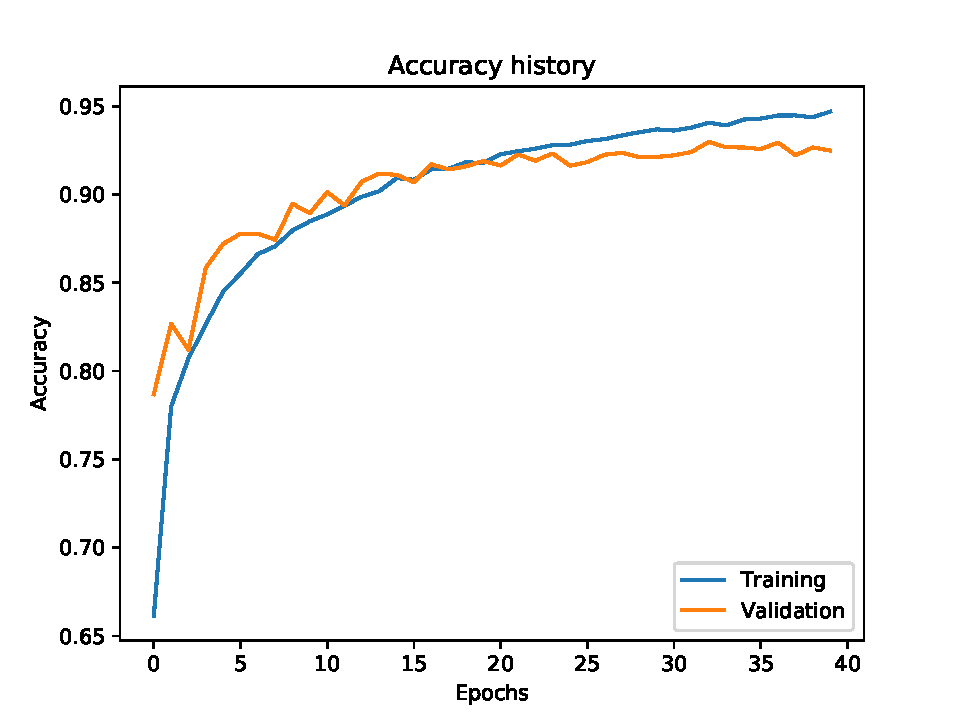
\includegraphics[width=.45\linewidth]{fig/Appendix_CNN/accuracyhistoryequal.pdf} \label{fig:accequal}}
  \end{subfigure}
 \begin{subfigure}[Gewichteter Datensatz]{
 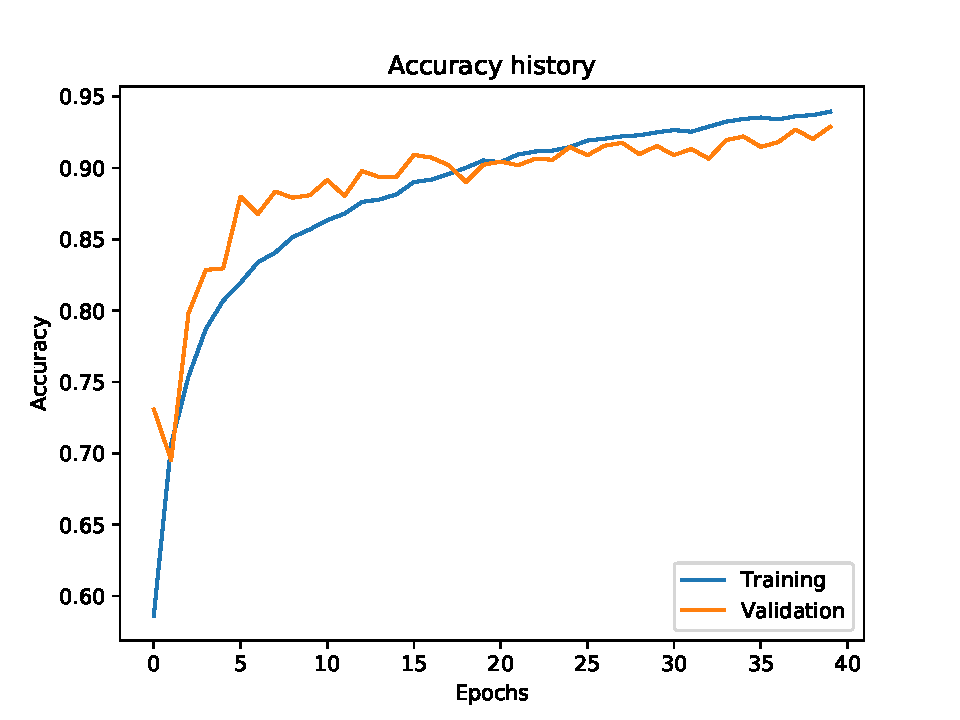
\includegraphics[width=.45\linewidth]{fig/Appendix_CNN/accuracyhistorynormal.pdf}\label{fig:accnormal}}
  \end{subfigure} \\
  \begin{subfigure}[relu statt elu als Aktivierungsfunktion]{
 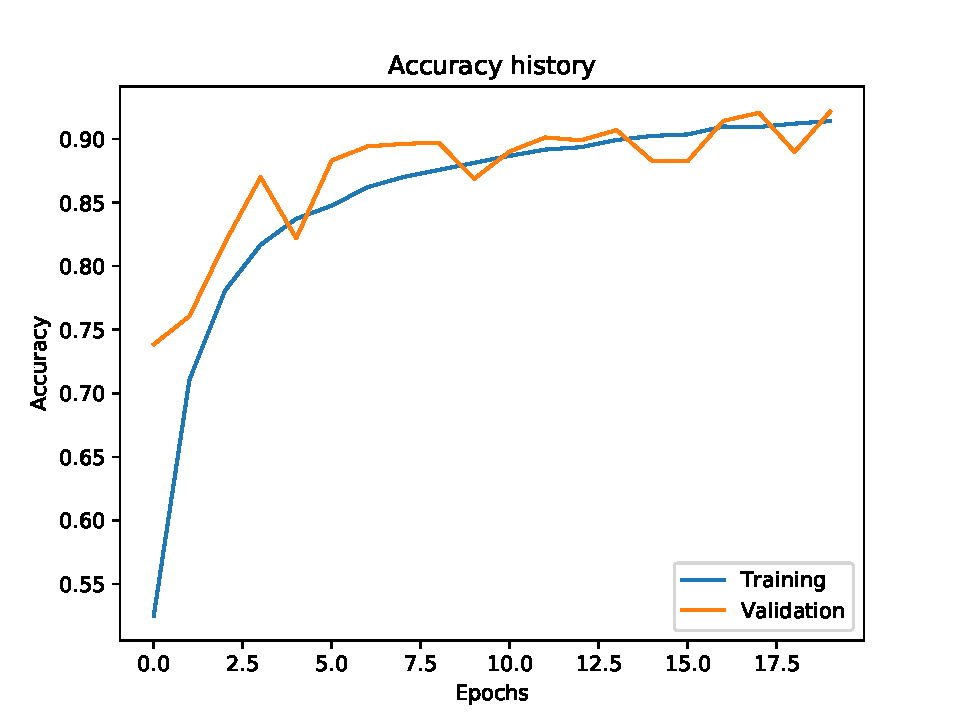
\includegraphics[width=.45\linewidth]{fig/Appendix_CNN/accuracyhistoryrelu.pdf}\label{fig:accrelu}}
  \end{subfigure}
 \begin{subfigure}[Verkleinerte Dimensionen der dichten Lagen]{
 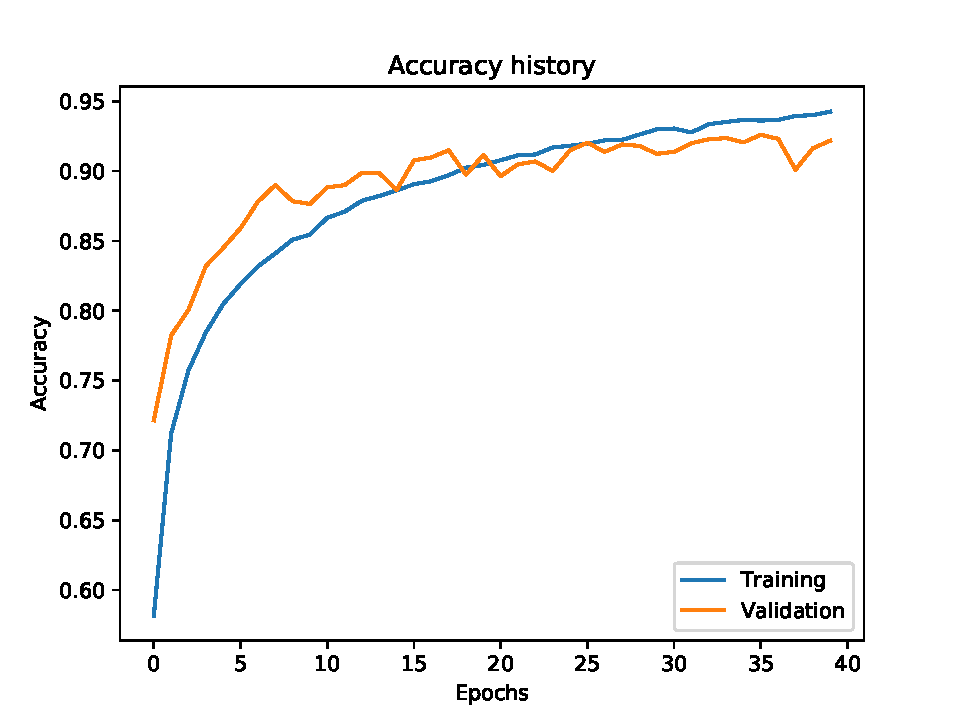
\includegraphics[width=.45\linewidth]{fig/Appendix_CNN/accuracyhistorysmaller.pdf}\label{fig:accsmaller2}}
  \end{subfigure}
  \caption{Werte der Genauigkeit nach jeder Epoche für das CNN mit der Referenzstruktur bei Propagation des ungewichteten Trainings- und Validierungsdatensatzes in \ref{fig:accequal} und bei Propagation des gewichteten Trainings- und Validierungsdatensatzes in \ref{fig:accnormal} sowie die entsprechenden Werte für die Verwendung der relu Funktion als Aktivierungsfunktion der versteckten Lagen in \ref{fig:accrelu} und bei Anpassung der Dimension der dichten Lagen in \ref{fig:accsmaller2}.}
\end{figure}

\setcounter{subfigure}{0}
\begin{figure}
 \centering
  \begin{subfigure}[Ungewichteter Datensatz]{
 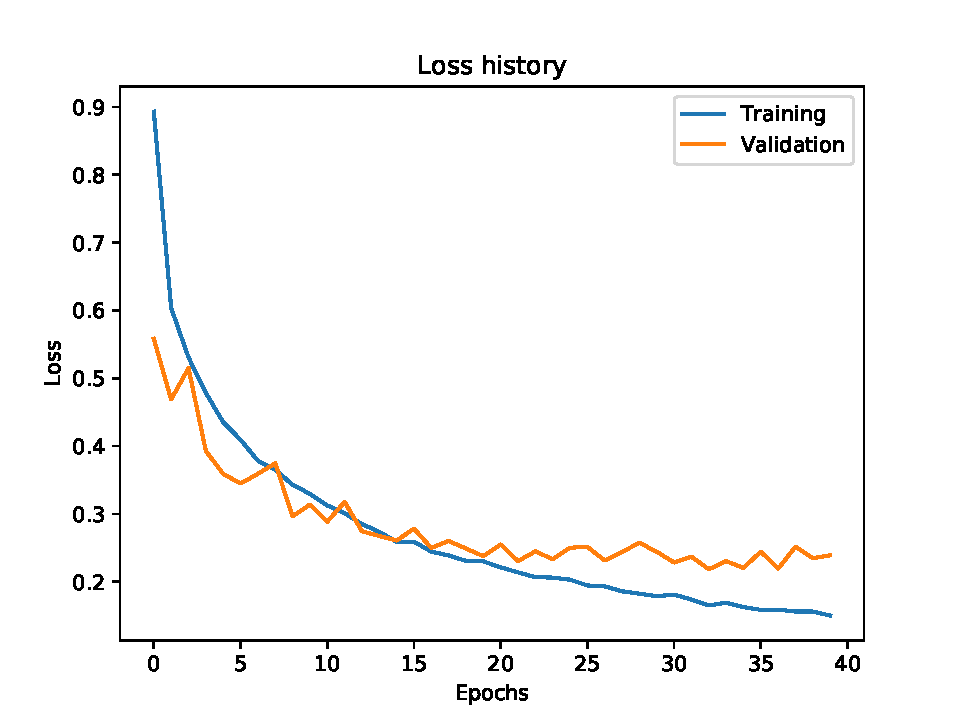
\includegraphics[width=.45\linewidth]{fig/Appendix_CNN/losshistoryequal.pdf} \label{fig:lossequal}}
  \end{subfigure}
 \begin{subfigure}[Gewichteter Datensatz]{
 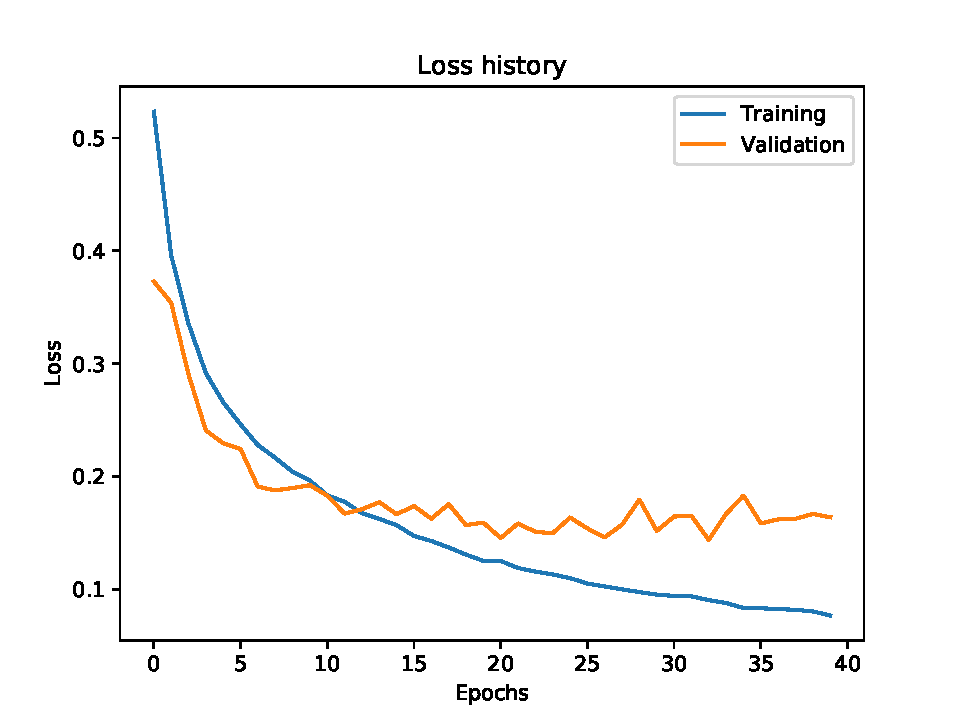
\includegraphics[width=.45\linewidth]{fig/Appendix_CNN/losshistorynormal.pdf}\label{fig:lossnormal}}
  \end{subfigure} \\
  \begin{subfigure}[relu statt elu als Aktivierungsfunktion]{
 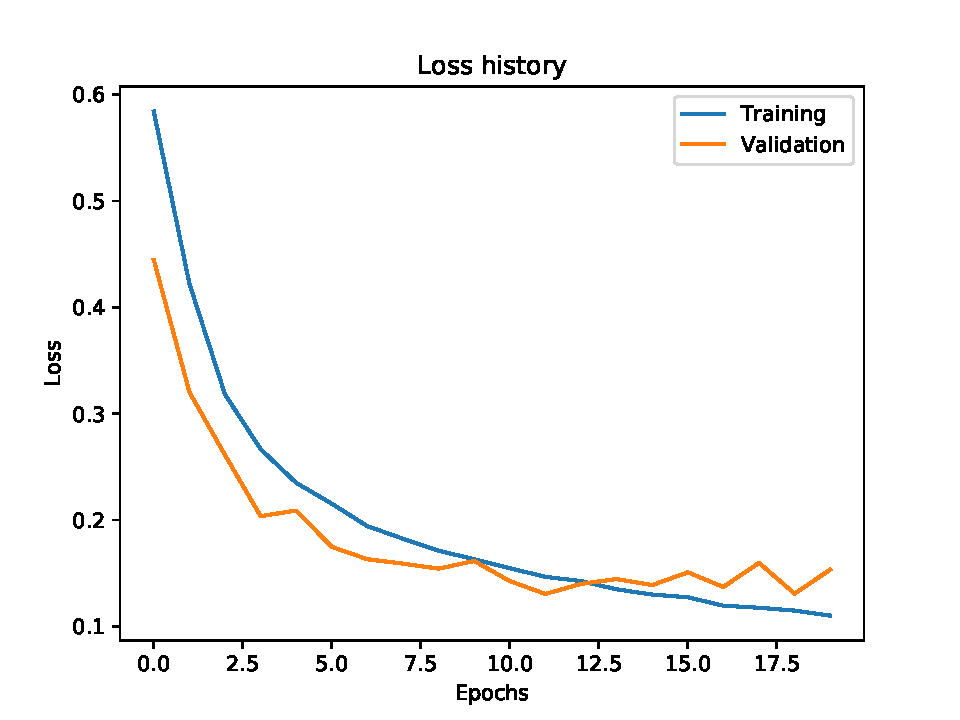
\includegraphics[width=.45\linewidth]{fig/Appendix_CNN/losshistoryrelu.pdf}\label{fig:lossrelu}}
  \end{subfigure}
 \begin{subfigure}[Verkleinerte Dimensionen der dichten Lagen]{
 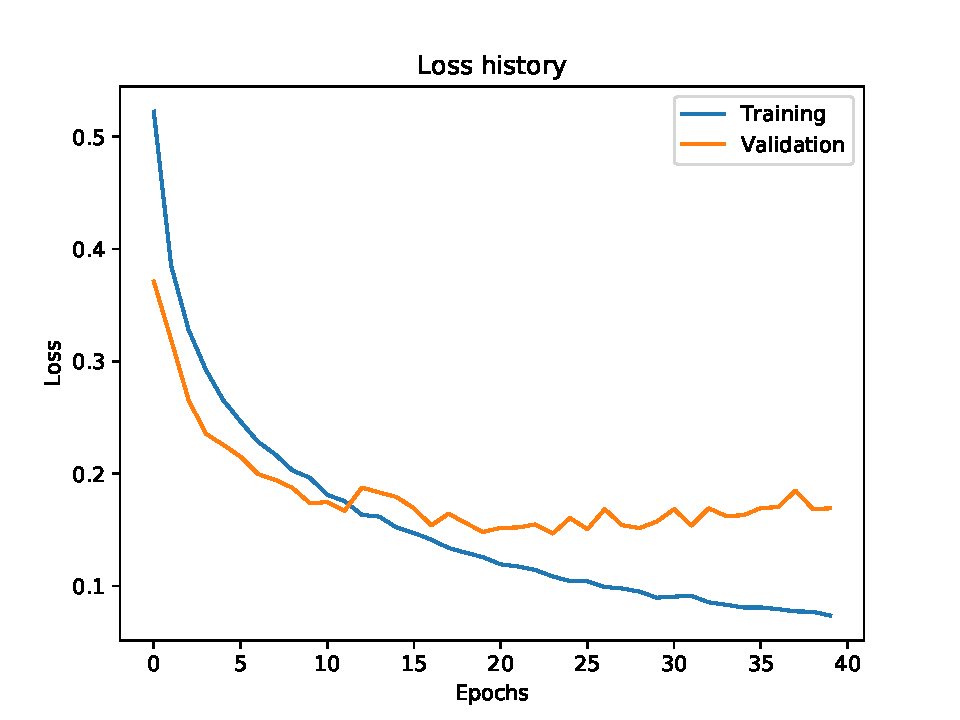
\includegraphics[width=.45\linewidth]{fig/Appendix_CNN/losshistorysmaller.pdf}\label{fig:losssmaller2}}
  \end{subfigure}
  \caption{Werte der Verlustfunktion nach jeder Epoche für das CNN mit der Referenzstruktur bei Propagation des ungewichteten Trainings- und Validierungsdatensatzes in \ref{fig:lossequal} und bei Propagation des gewichteten Trainings- und Validierungsdatensatzes in \ref{fig:lossnormal} sowie die entsprechenden Werte für die Verwendung der relu Funktion als Aktivierungsfunktion der versteckten Lagen in \ref{fig:lossrelu} und bei Anpassung der Dimension der dichten Lagen in \ref{fig:losssmaller2}.}
\end{figure}
\setcounter{subfigure}{0}



\begin{figure}
 \centering
  \begin{subfigure}[Ungewichteter Datensatz]{
 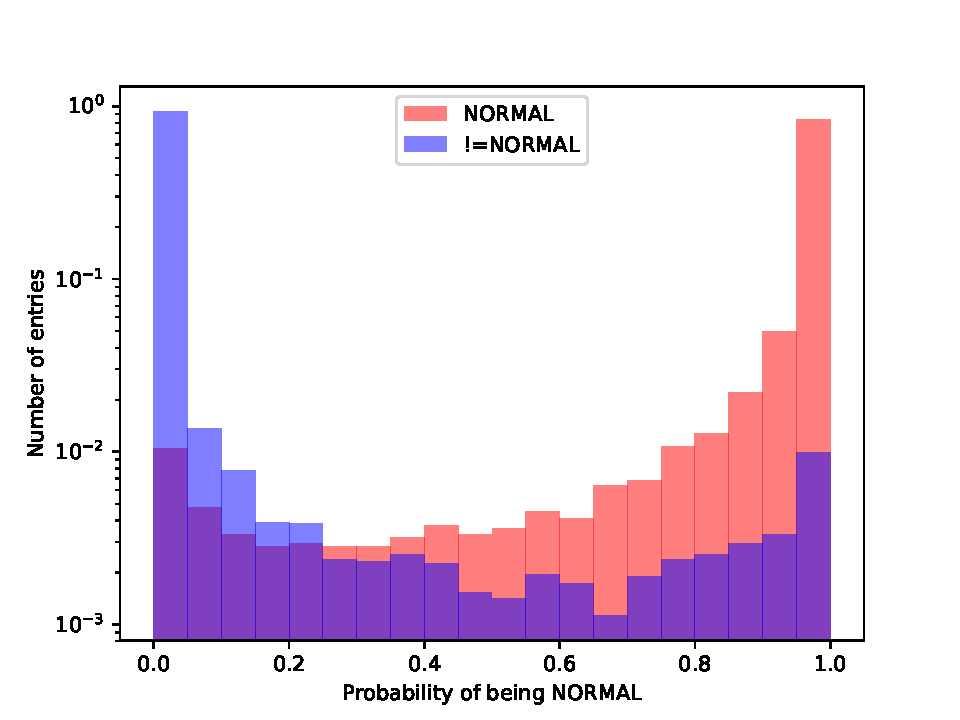
\includegraphics[width=.45\linewidth]{fig/Appendix_CNN/NORMALornotlogequal.pdf} \label{fig:NORMALequal}}
  \end{subfigure}
 \begin{subfigure}[Gewichteter Datensatz]{
 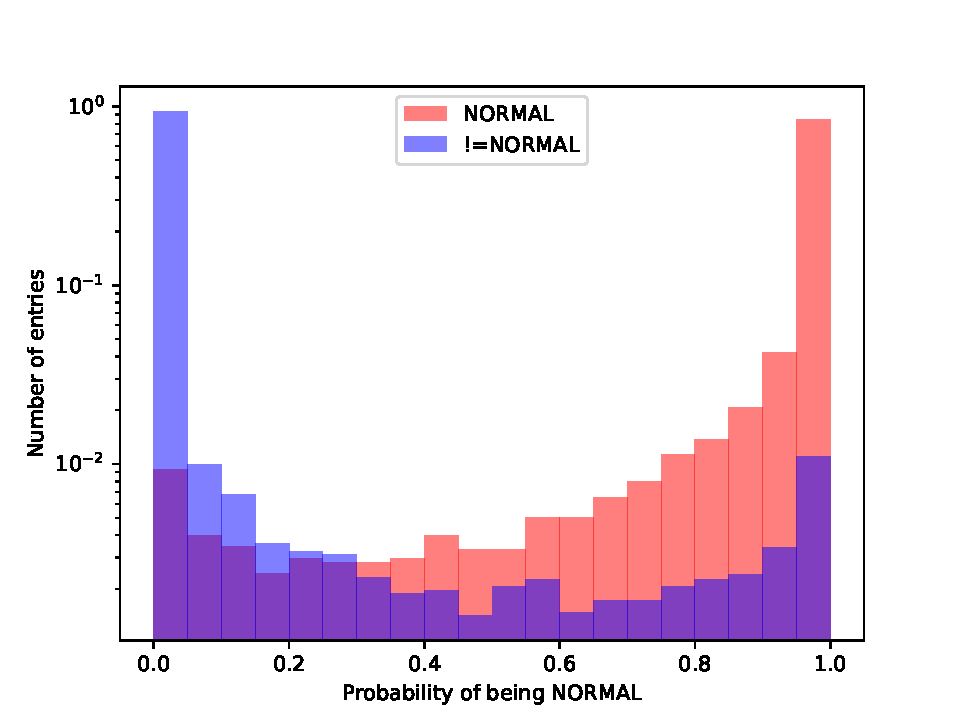
\includegraphics[width=.45\linewidth]{fig/Appendix_CNN/NORMALornotlognormal.pdf}\label{fig:NORMALnormal}}
  \end{subfigure} \\
  \begin{subfigure}[relu statt elu als Aktivierungsfunktion]{
 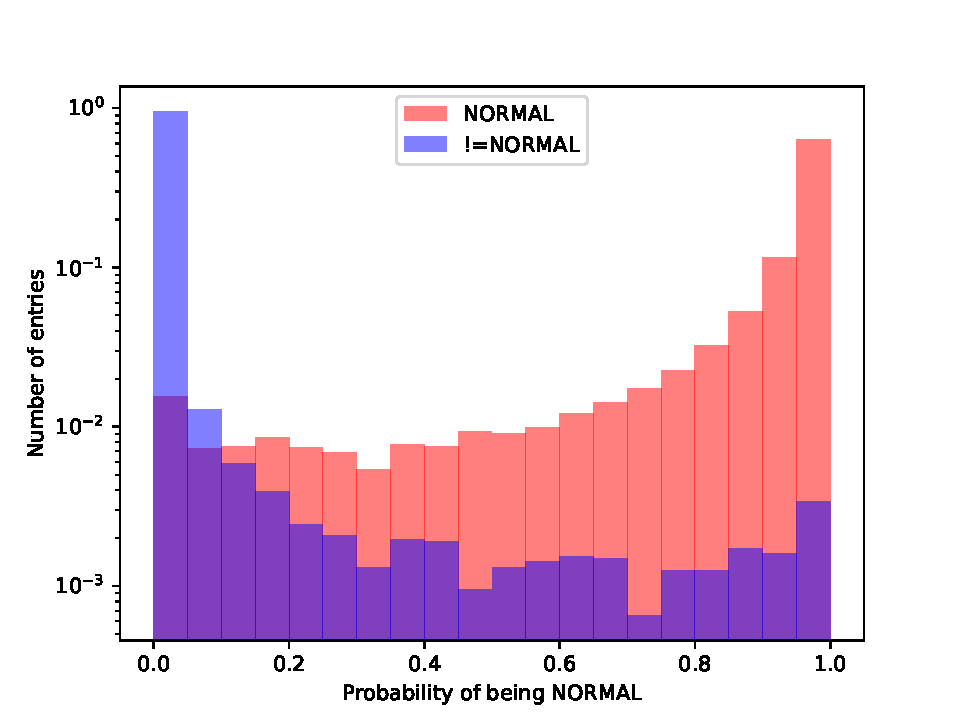
\includegraphics[width=.45\linewidth]{fig/Appendix_CNN/NORMALornotlogrelu.pdf}\label{fig:NORMALrelu}}
  \end{subfigure}
 \begin{subfigure}[Verkleinerte Dimensionen der dichten Lagen]{
 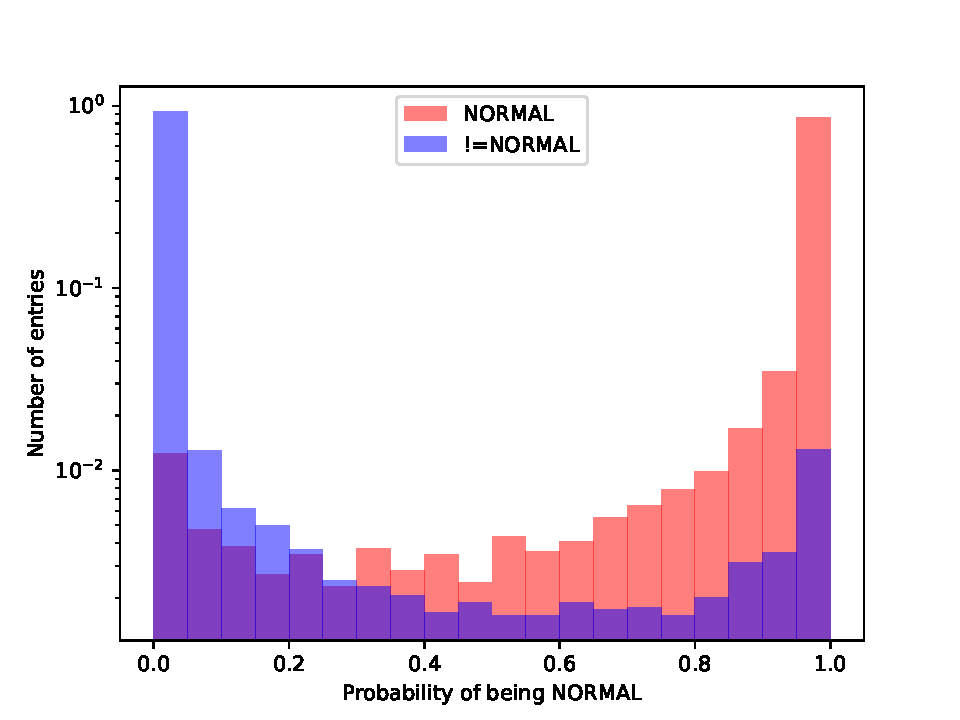
\includegraphics[width=.45\linewidth]{fig/Appendix_CNN/NORMALornotlogsmaller.pdf}\label{fig:NORMALsmaller}}
  \end{subfigure}
  \caption{Verteilung der von dem CNN vorhergesagten Wahrscheinlichkeiten für die Aufnahmen der Klasse NORMAL und die Aufnahmen au{\ss}erhalb der Klasse NORMAL (!=NORMAL) der Klasse NORMAL anzugehören für das CNN mit der Referenzstruktur bei Propagation des ungewichteten Trainings- und Validierungsdatensatzes in \ref{fig:NORMALequal} und bei Propagation des gewichteten Trainings- und Validierungsdatensatzes in \ref{fig:NORMALnormal} sowie die entsprechenden Werte für die Verwendung der relu Funktion als Aktivierungsfunktion der versteckten Lagen in \ref{fig:NORMALrelu} und bei Anpassung der Dimension der dichten Lagen in \ref{fig:NORMALsmaller}.}
\end{figure}
\setcounter{subfigure}{0}


\begin{figure}
 \centering
  \begin{subfigure}[Ungewichteter Datensatz]{
 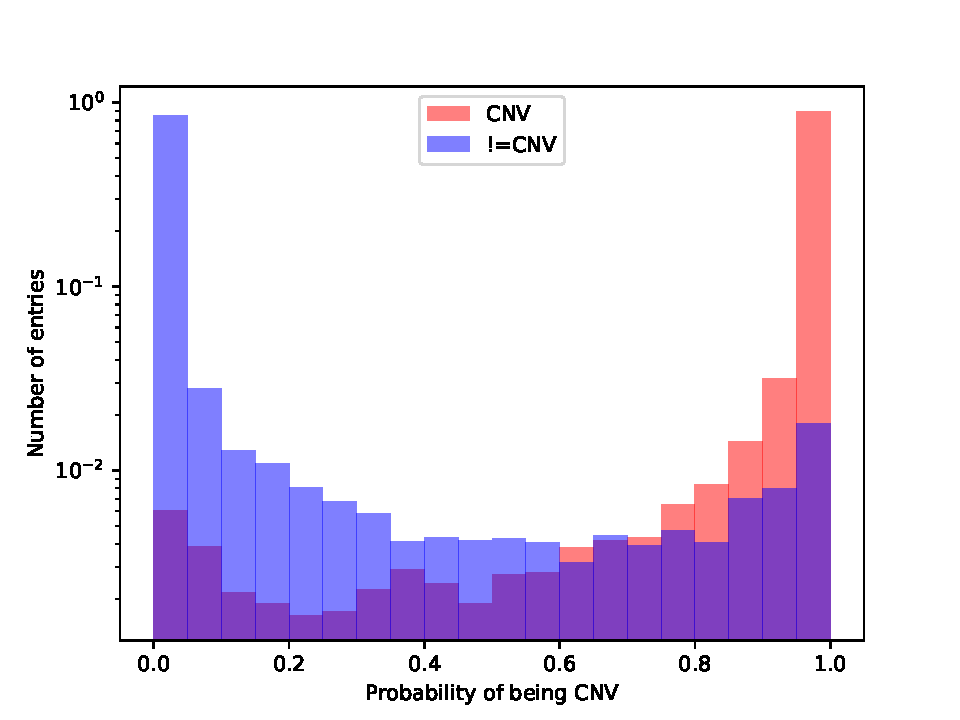
\includegraphics[width=.45\linewidth]{fig/Appendix_CNN/CNVornotlogequal.pdf} \label{fig:CNVequal}}
  \end{subfigure}
 \begin{subfigure}[Gewichteter Datensatz]{
 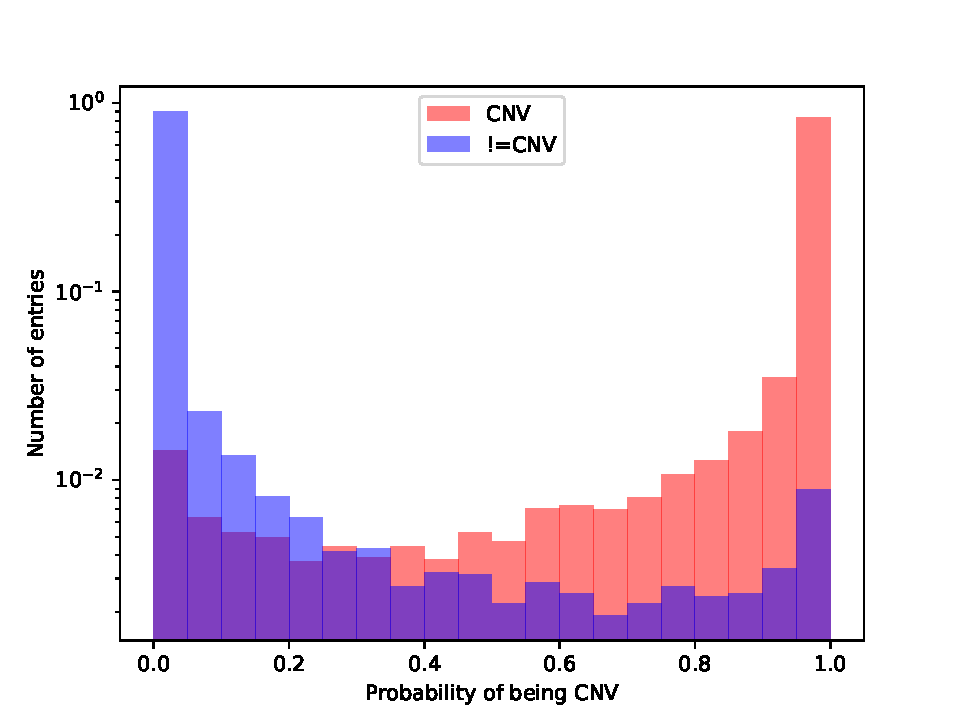
\includegraphics[width=.45\linewidth]{fig/Appendix_CNN/CNVornotlognormal.pdf}\label{fig:CNVnormal}}
  \end{subfigure} \\
  \begin{subfigure}[relu statt elu als Aktivierungsfunktion]{
 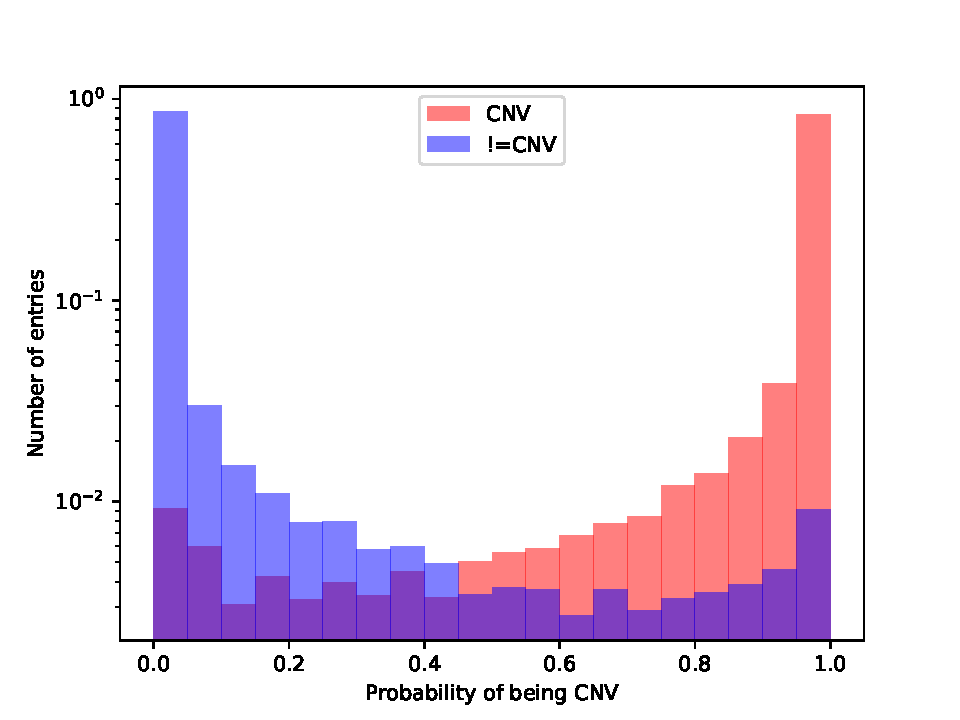
\includegraphics[width=.45\linewidth]{fig/Appendix_CNN/CNVornotlogrelu.pdf}\label{fig:CNVrelu}}
  \end{subfigure}
 \begin{subfigure}[Verkleinerte Dimensionen der dichten Lagen]{
 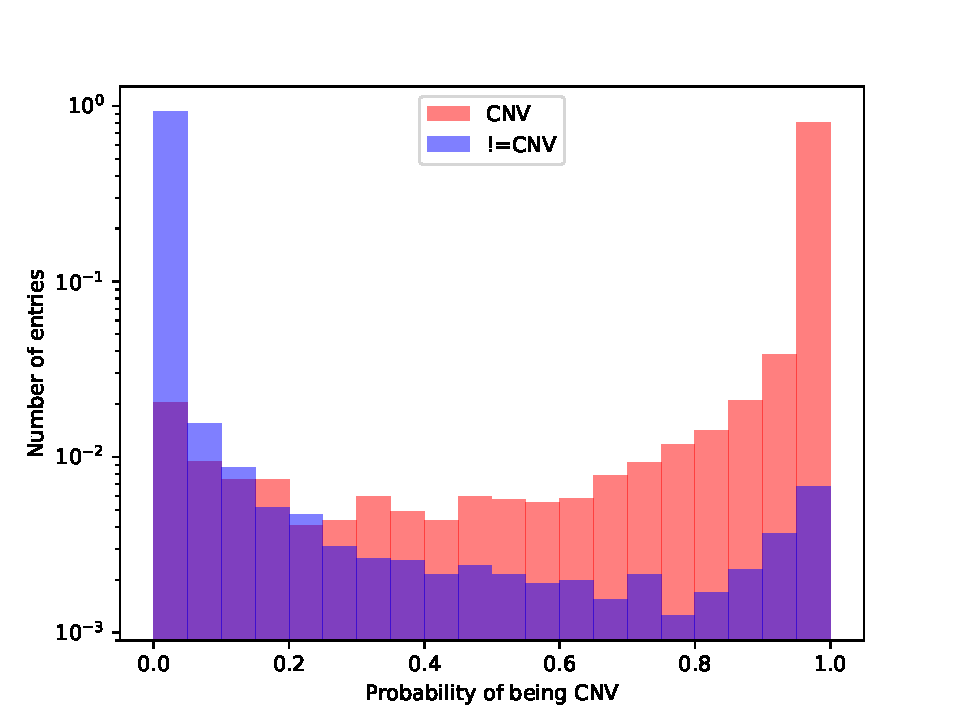
\includegraphics[width=.45\linewidth]{fig/Appendix_CNN/CNVornotlogsmaller.pdf}\label{fig:CNVsmaller}}
  \end{subfigure}
  \caption{Verteilung der von dem CNN vorhergesagten Wahrscheinlichkeiten für die Aufnahmen der Klasse CNV und die Aufnahmen außerhalb der Klasse CNV (!=CNV) der Klasse CNV anzugehören für das CNN mit der Referenzstruktur bei Propagation des ungewichteten Trainings- und Validierungsdatensatzes in \ref{fig:CNVequal} und bei Propagation des gewichteten Trainings- und Validierungsdatensatzes in \ref{fig:CNVnormal} sowie die entsprechenden Werte für die Verwendung der relu Funktion als Aktivierungsfunktion der versteckten Lagen in \ref{fig:CNVrelu} und bei Anpassung der Dimension der dichten Lagen in \ref{fig:CNVsmaller}.}
\end{figure}
\setcounter{subfigure}{0}



\begin{figure}
 \centering
  \begin{subfigure}[Ungewichteter Datensatz]{
 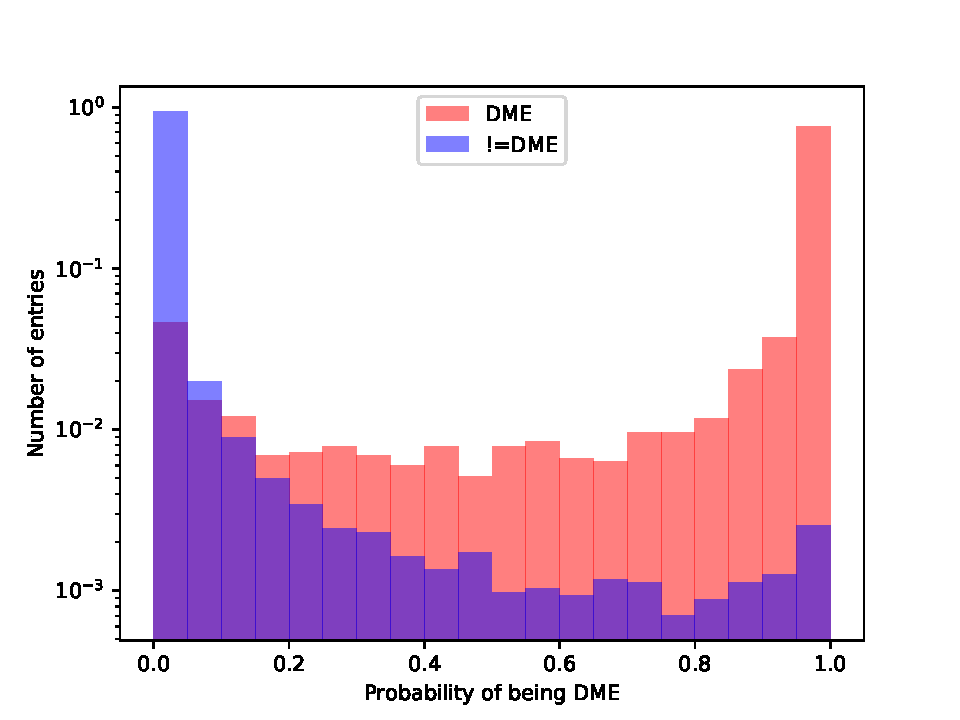
\includegraphics[width=.45\linewidth]{fig/Appendix_CNN/DMEornotlogequal.pdf} \label{fig:DMEequal}}
  \end{subfigure}
 \begin{subfigure}[Gewichteter Datensatz]{
 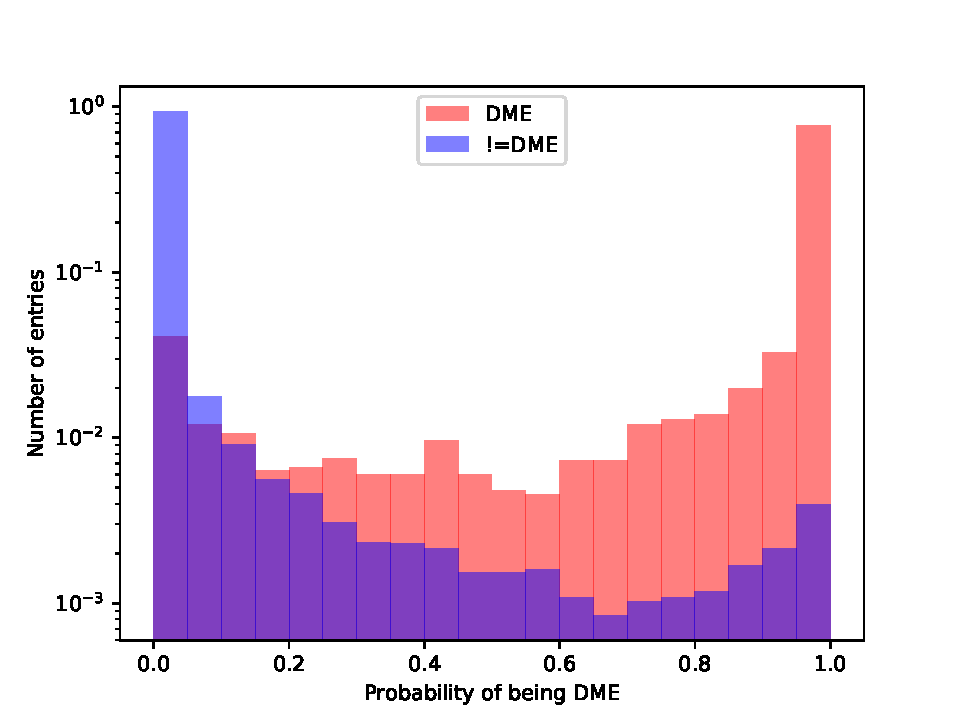
\includegraphics[width=.45\linewidth]{fig/Appendix_CNN/DMEornotlognormal.pdf}\label{fig:DMEnormal}}
  \end{subfigure} \\
  \begin{subfigure}[relu statt elu als Aktivierungsfunktion]{
 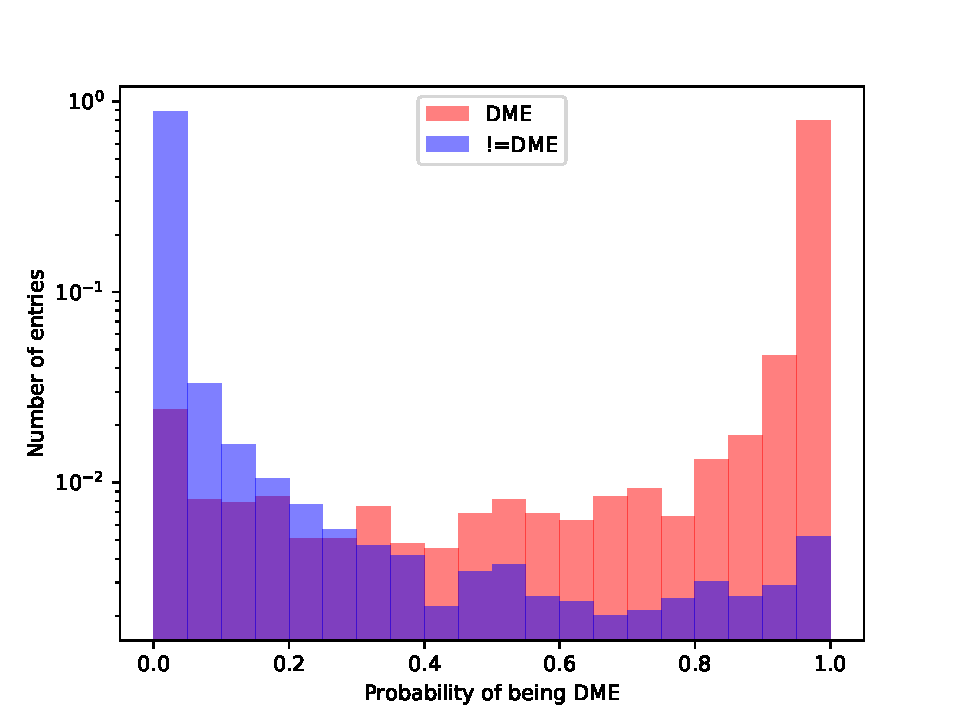
\includegraphics[width=.45\linewidth]{fig/Appendix_CNN/DMEornotlogrelu.pdf}\label{fig:DMErelu}}
  \end{subfigure}
 \begin{subfigure}[Verkleinerte Dimensionen der dichten Lagen]{
 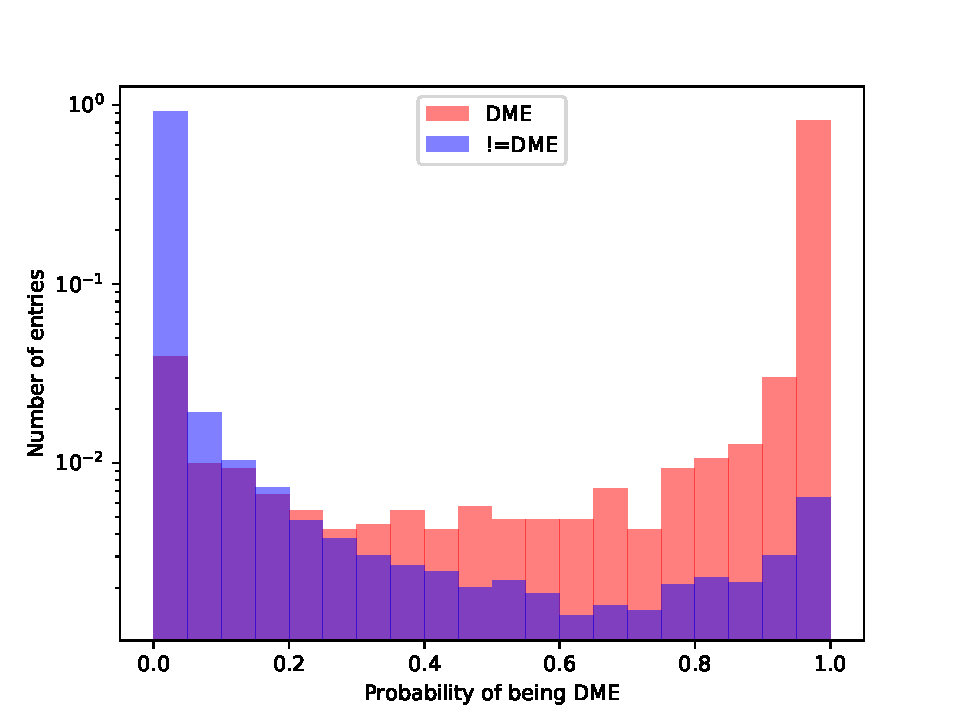
\includegraphics[width=.45\linewidth]{fig/Appendix_CNN/DMEornotlogsmaller.pdf}\label{fig:DMEsmaller}}
  \end{subfigure}
  \caption{Verteilung der von dem CNN vorhergesagten Wahrscheinlichkeiten für die Aufnahmen der Klasse DME und die Aufnahmen außerhalb der Klasse DME (!=DME) der Klasse DME anzugehören für das CNN mit der Referenzstruktur bei Propagation des ungewichteten Trainings- und Validierungsdatensatzes in \ref{fig:DMEequal} und bei Propagation des gewichteten Trainings- und Validierungsdatensatzes in \ref{fig:DMEnormal} sowie die entsprechenden Werte für die Verwendung der relu Funktion als Aktivierungsfunktion der versteckten Lagen in \ref{fig:DMErelu} und bei Anpassung der Dimension der dichten Lagen in \ref{fig:DMEsmaller}.}
\end{figure}
\setcounter{subfigure}{0}



\begin{figure}
 \centering
  \begin{subfigure}[Ungewichteter Datensatz]{
 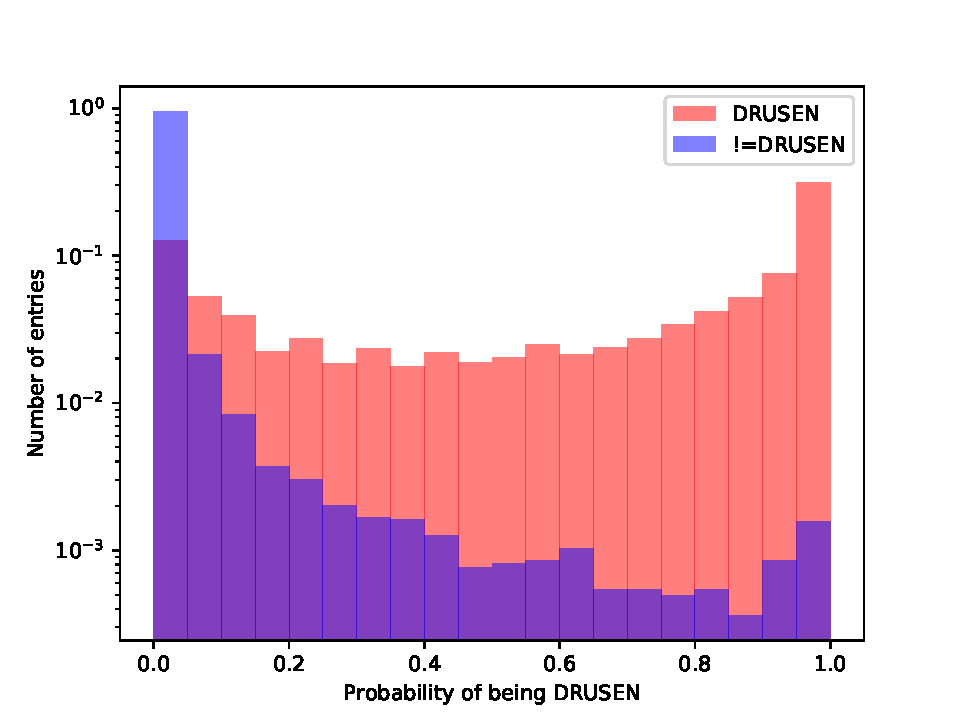
\includegraphics[width=.45\linewidth]{fig/Appendix_CNN/DRUSENornotlogequal.pdf} \label{fig:DRUSENequal}}
  \end{subfigure}
 \begin{subfigure}[Gewichteter Datensatz]{
 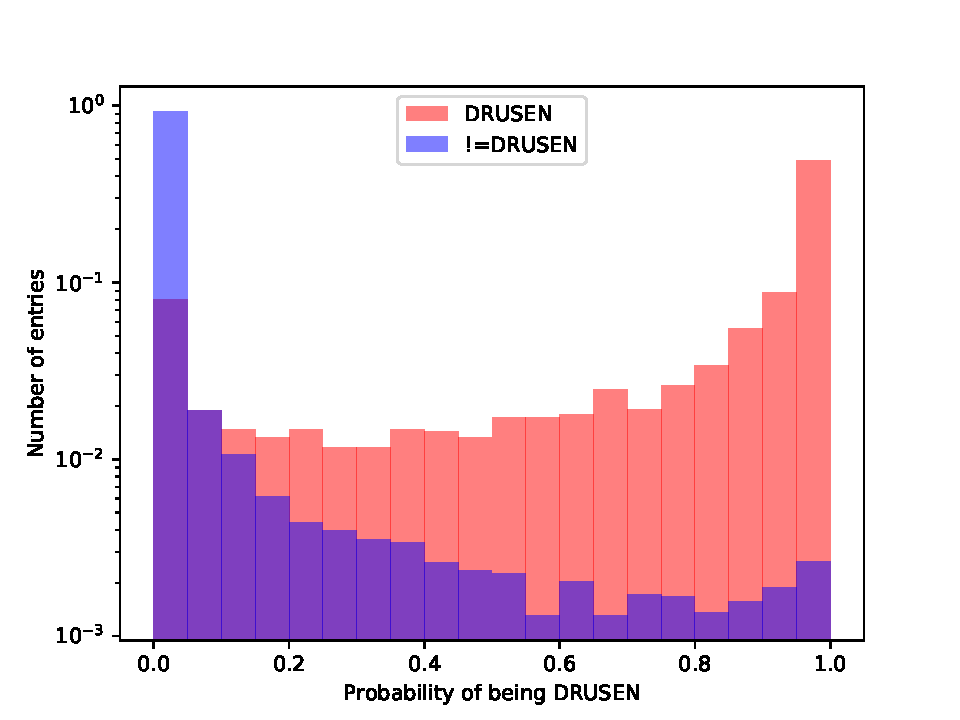
\includegraphics[width=.45\linewidth]{fig/Appendix_CNN/DRUSENornotlognormal.pdf}\label{fig:DRUSENnormal}}
  \end{subfigure} \\
  \begin{subfigure}[relu statt elu als Aktivierungsfunktion]{
 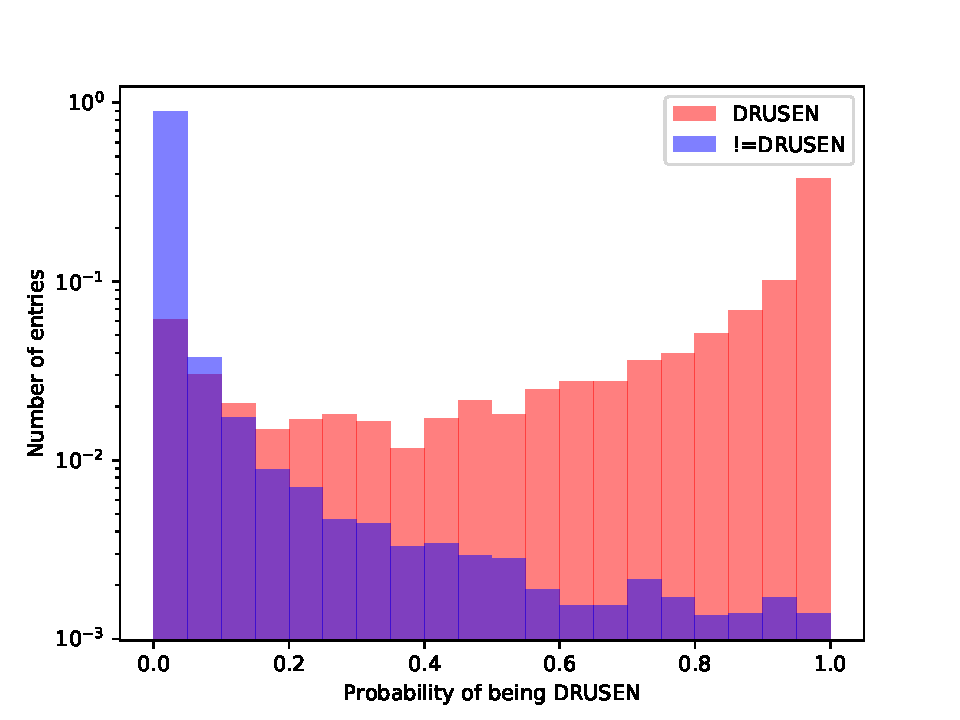
\includegraphics[width=.45\linewidth]{fig/Appendix_CNN/DRUSENornotlogrelu.pdf}\label{fig:DRUSENrelu}}
  \end{subfigure}
 \begin{subfigure}[Verkleinerte Dimensionen der dichten Lagen]{
 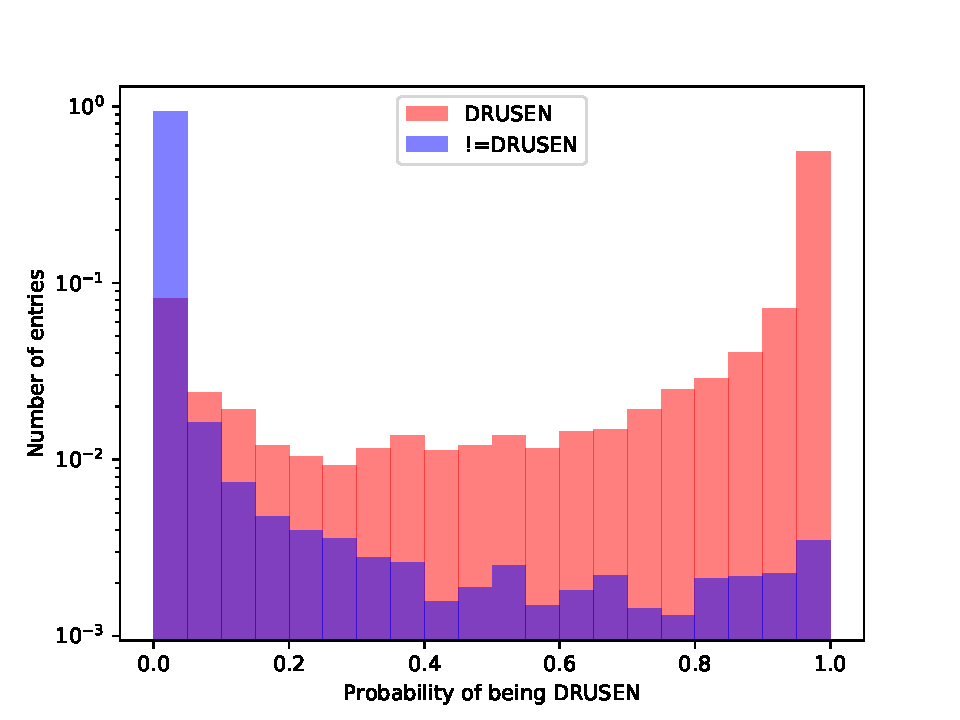
\includegraphics[width=.45\linewidth]{fig/Appendix_CNN/DRUSENornotlogsmaller.pdf}\label{fig:DRUSENsmaller}}
  \end{subfigure}
  \caption{Verteilung der von dem CNN vorhergesagten Wahrscheinlichkeiten für die Aufnahmen der Klasse DRUSEN und die Aufnahmen außerhalb der Klasse DRUSEN (!=DRUSEN) der Klasse DRUSEN anzugehören für das CNN mit der Referenzstruktur bei Propagation des ungewichteten Trainings- und Validierungsdatensatzes in \ref{fig:DRUSENequal} und bei Propagation des gewichteten Trainings- und Validierungsdatensatzes in \ref{fig:DRUSENnormal} sowie die entsprechenden Werte für die Verwendung der relu Funktion als Aktivierungsfunktion der versteckten Lagen in \ref{fig:DRUSENrelu} und bei Anpassung der Dimension der dichten Lagen in \ref{fig:DRUSENsmaller}.}
\end{figure}
\setcounter{subfigure}{0}



\clearpage


\section{Zusatzliche Abbildungen und Ergebnisse zur Optimierungsstudie des DNN}



\begin{figure}
 \centering
  \begin{subfigure}[Genauigkeit]{
 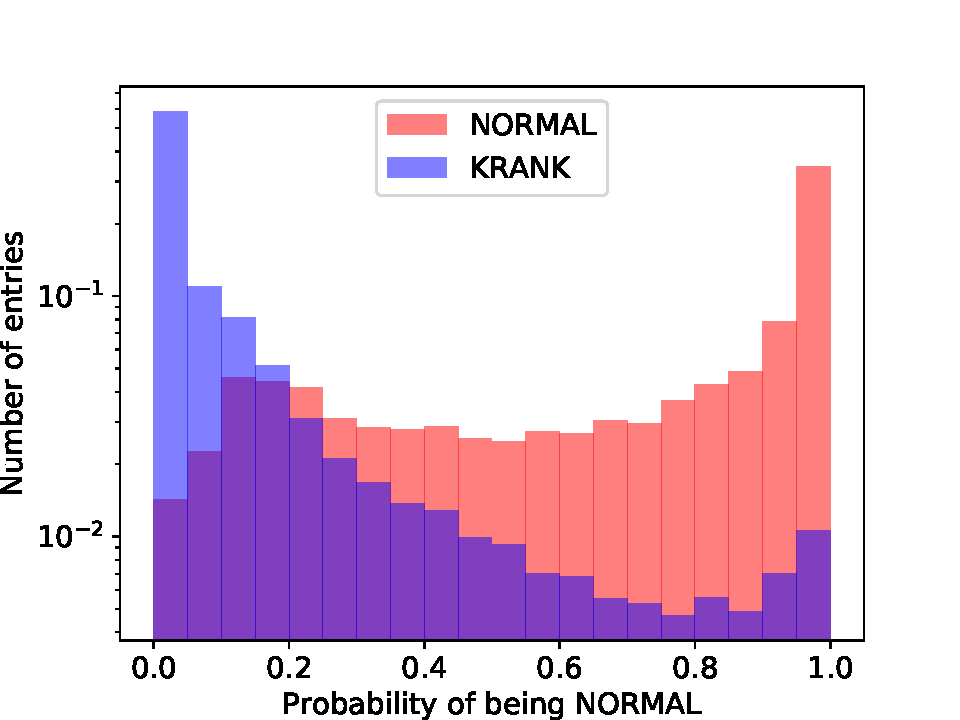
\includegraphics[width=.45\linewidth]{fig/Appendix_DNN/NORMALornotlog6test.pdf} \label{fig:testnorm}}
  \end{subfigure}
 \begin{subfigure}[Verlustfunktion]{
 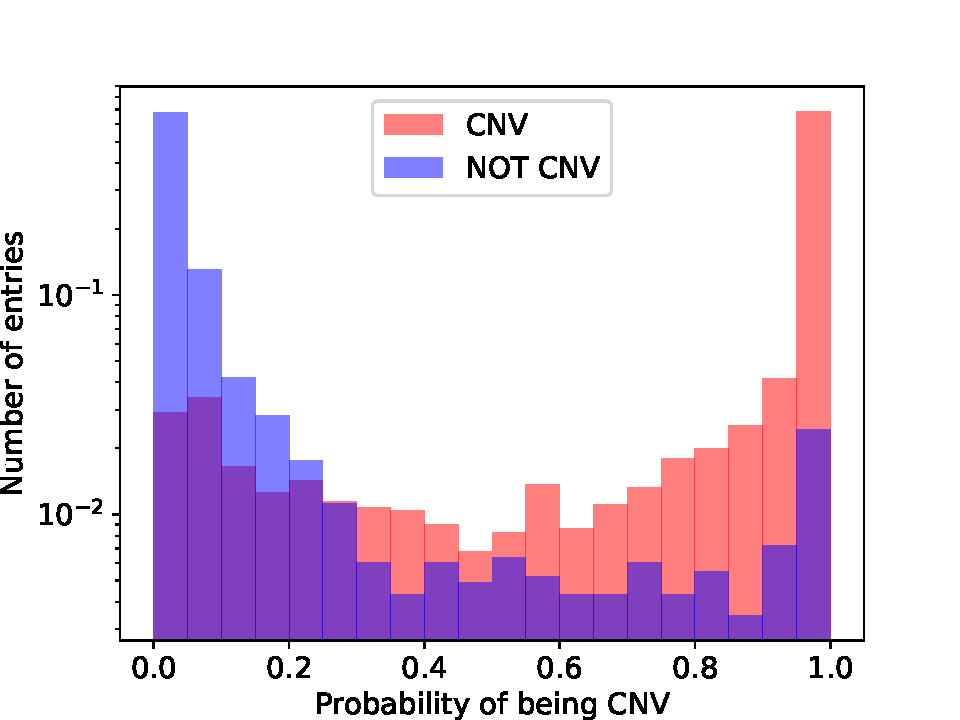
\includegraphics[width=.45\linewidth]{fig/Appendix_DNN/CNVornotlog6test.pdf}\label{fig:testcnv}}
  \end{subfigure} \\
  \begin{subfigure}[Genauigkeit]{
 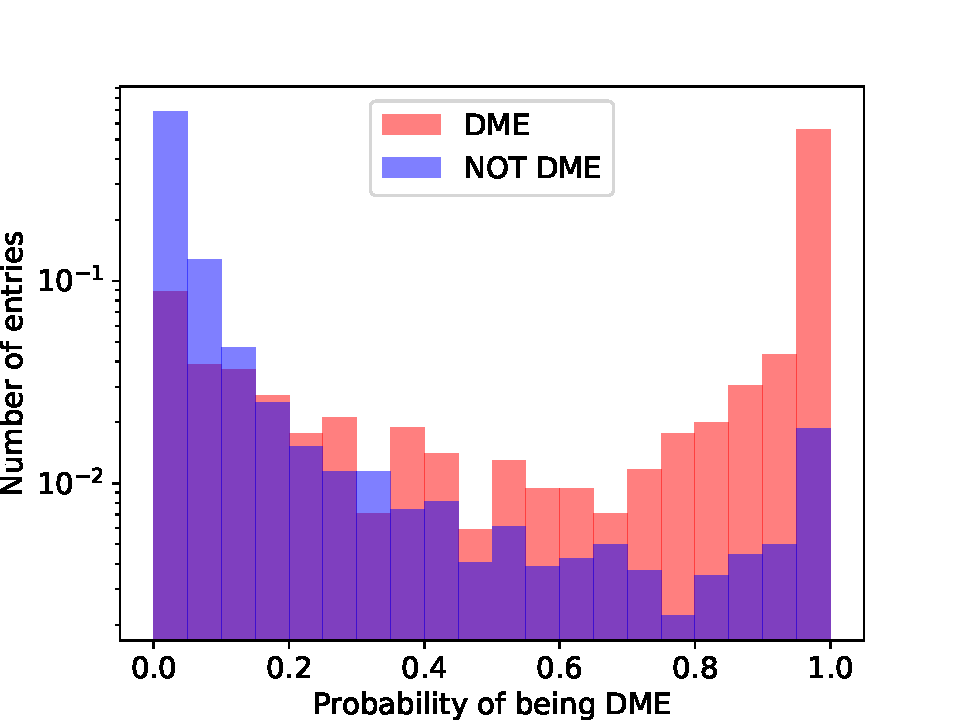
\includegraphics[width=.45\linewidth]{fig/Appendix_DNN/DMEornotlog6test.pdf}\label{fig:testdme}}
  \end{subfigure}
 \begin{subfigure}[Verlustfunktion]{
 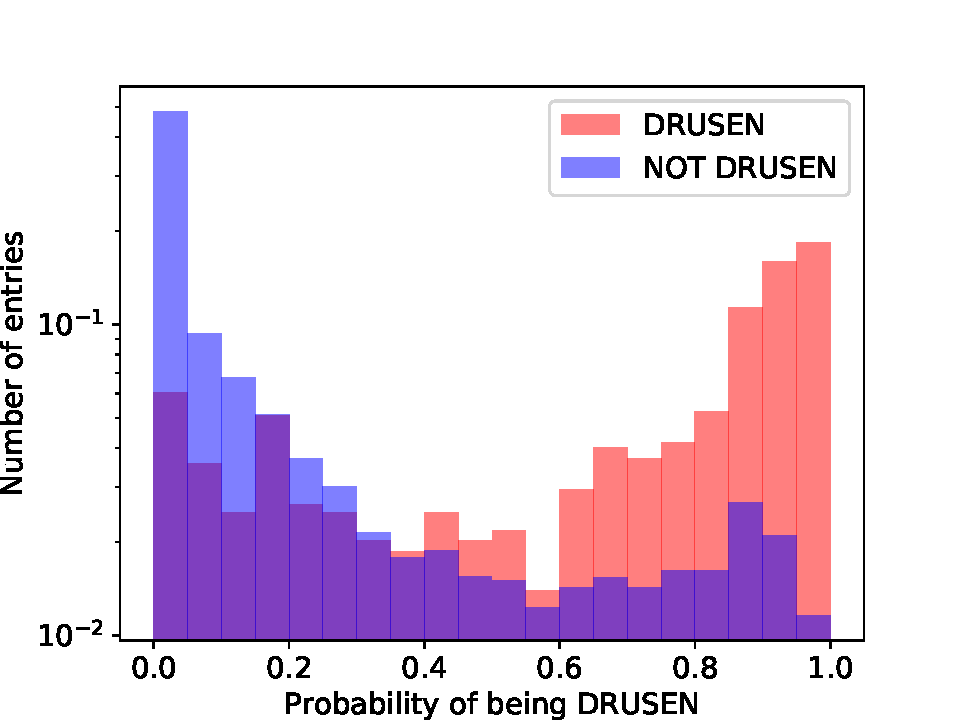
\includegraphics[width=.45\linewidth]{fig/Appendix_DNN/DRUSENornotlog6test.pdf}\label{fig:testdrusen}}
  \end{subfigure}
  \caption{Verteilung der von dem CNN vorhergesagten Wahrscheinlichkeiten unter Verwendung des Testdatensatzes für die Aufnahmen innerhalb einer Klasse X und für die Aufnahmen, die nicht dieser Klasse angehören (!=X), der Klasse X anzugehören. Die Abbildungen \ref{fig:testnorm}, \ref{fig:testcnv}, \ref{fig:testdme} und \ref{fig:testdrusen} zeigen dies für die Klassen NORMAL, CNV, DME respektive DRUSEN.}
\end{figure}

\setcounter{subfigure}{0}

\begin{figure}
 \centering
  \begin{subfigure}[Genauigkeit]{
 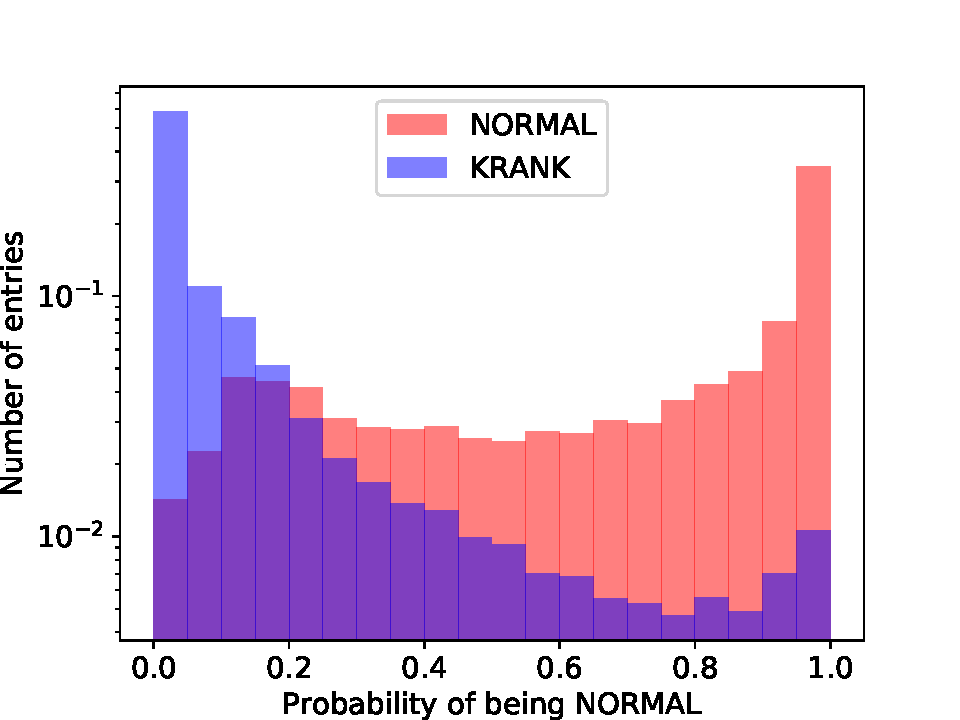
\includegraphics[width=.45\linewidth]{fig/Appendix_DNN/NORMALornotlog6.pdf} \label{fig:valnorm}}
  \end{subfigure}
 \begin{subfigure}[Verlustfunktion]{
 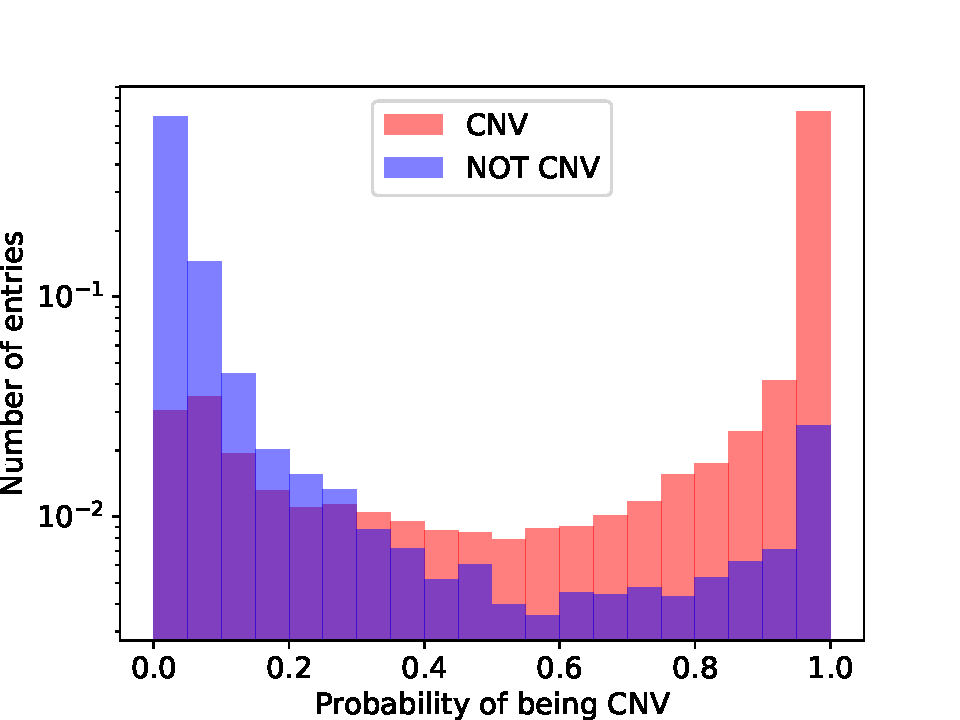
\includegraphics[width=.45\linewidth]{fig/Appendix_DNN/CNVornotlog6.pdf}\label{fig:valcnv}}
  \end{subfigure} \\
  \begin{subfigure}[Genauigkeit]{
 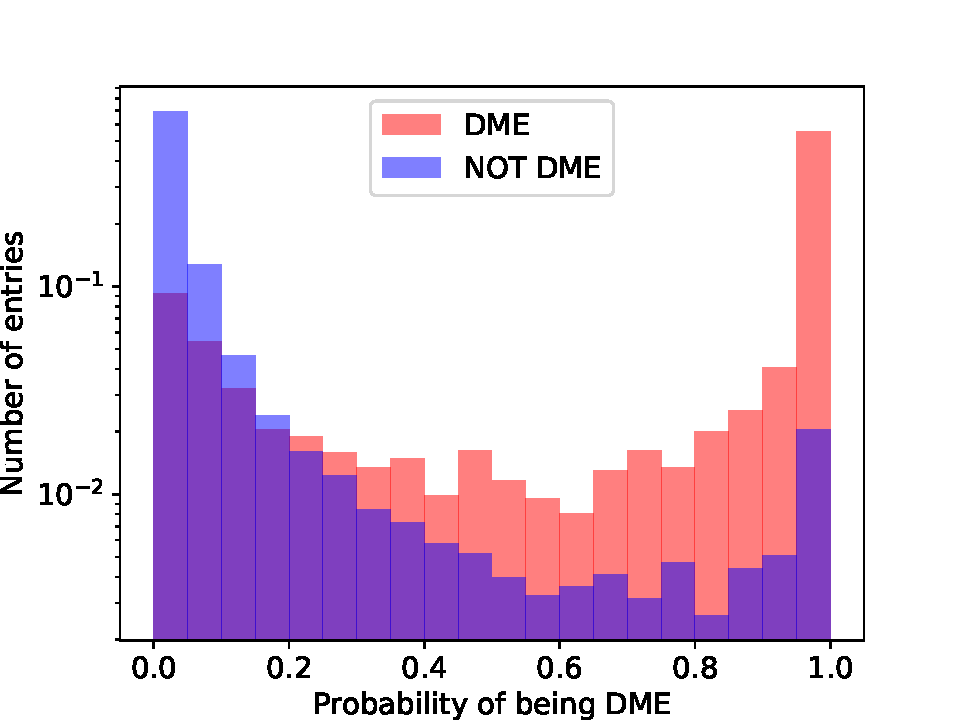
\includegraphics[width=.45\linewidth]{fig/Appendix_DNN/DMEornotlog6.pdf}\label{fig:valdme}}
  \end{subfigure}
 \begin{subfigure}[Verlustfunktion]{
 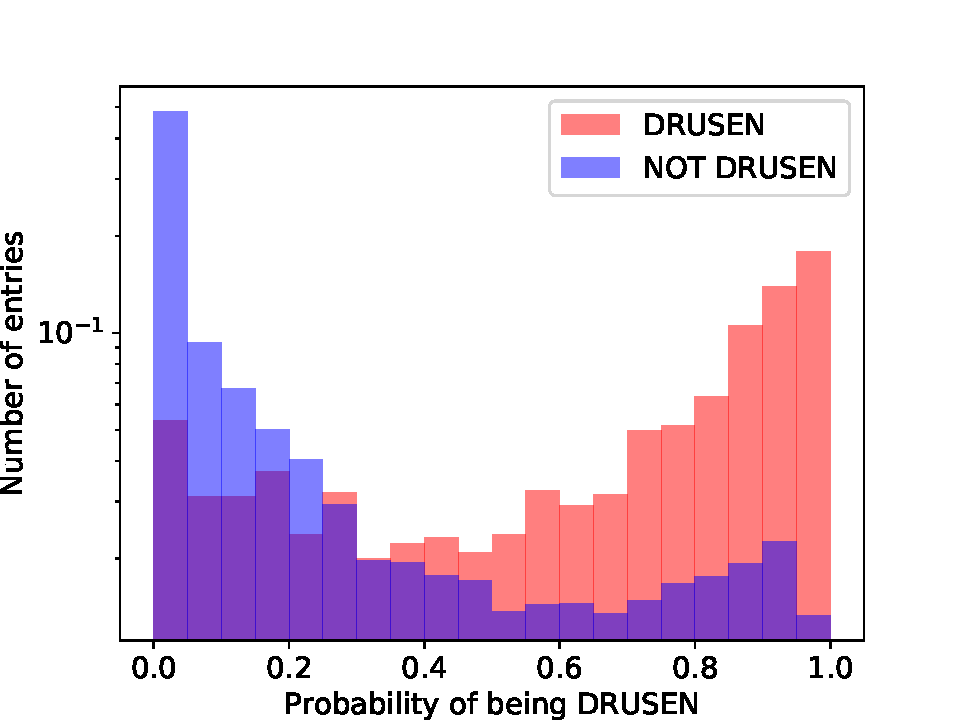
\includegraphics[width=.45\linewidth]{fig/Appendix_DNN/DRUSENornotlog6.pdf}\label{fig:valdrusen}}
  \end{subfigure}
  \caption{Verteilung der von dem CNN vorhergesagten Wahrscheinlichkeiten unter Verwendung des Validierungsdatensatzes für die Aufnahmen innerhalb einer Klasse X und für die Aufnahmen, die nicht dieser Klasse angehören (!=X), der Klasse X anzugehören. Die Abbildungen \ref{fig:valnorm}, \ref{fig:valcnv}, \ref{fig:valdme} und \ref{fig:valdrusen} zeigen dies für die Klassen NORMAL, CNV, DME respektive DRUSEN.}
\end{figure}

\setcounter{subfigure}{0}

\begin{figure}[!t]
\centering
\begin{subfigure}[Normal]{
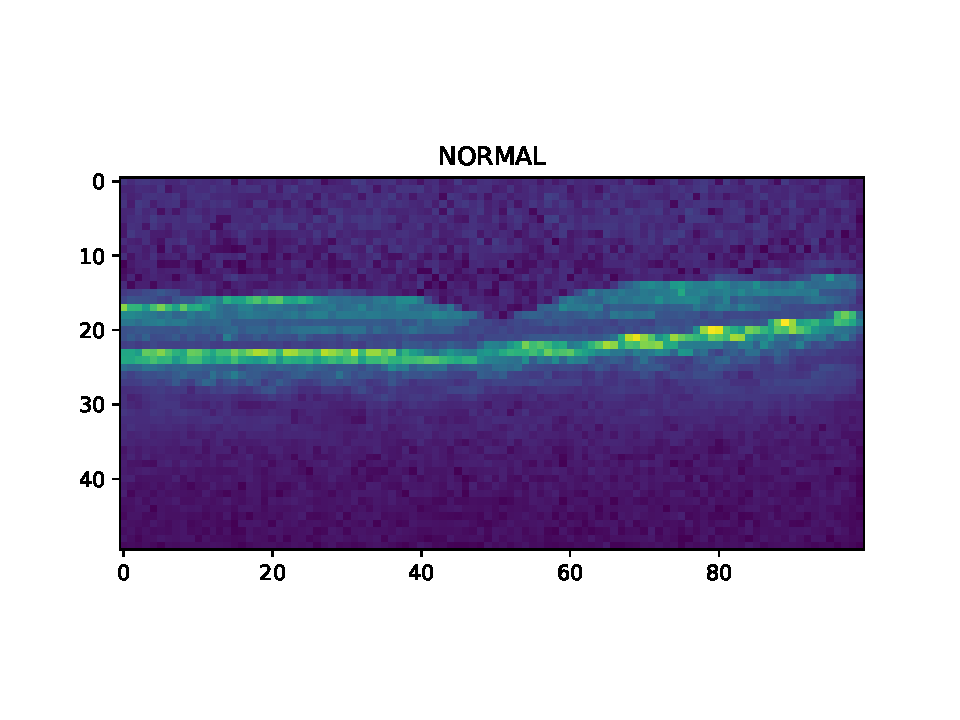
\includegraphics[width=.40\linewidth]{fig/Appendix_DNN/imageNORMALscan.pdf}}
\end{subfigure}%
\begin{subfigure}[Normal]{
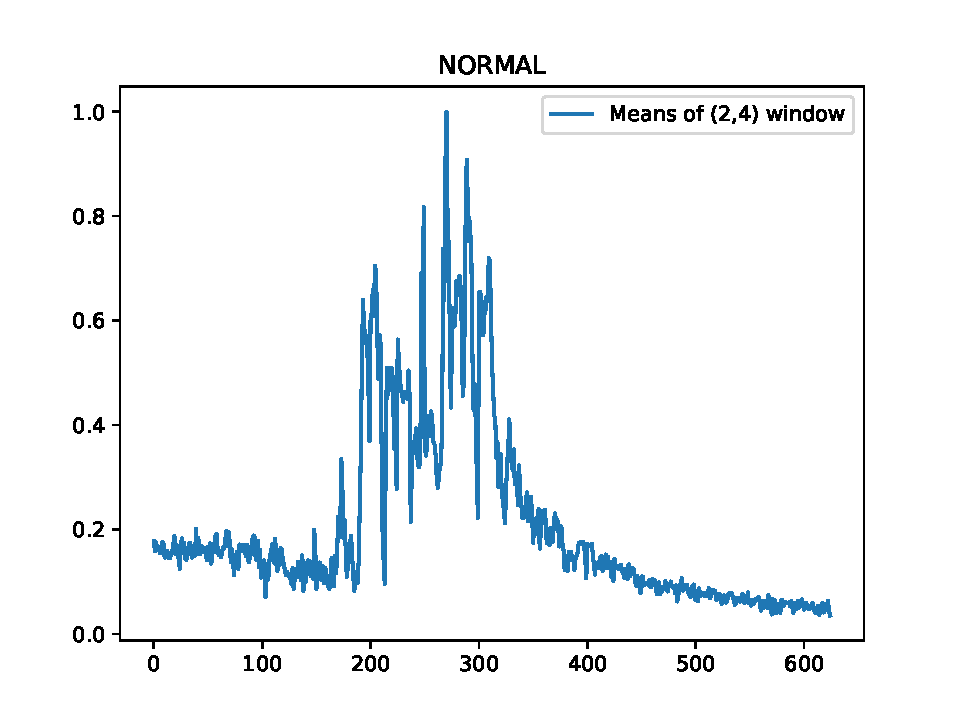
\includegraphics[width=.40\linewidth]{fig/Appendix_DNN/imageNORMALmeans.pdf}}
\end{subfigure}\\
\begin{subfigure}[CNV]{
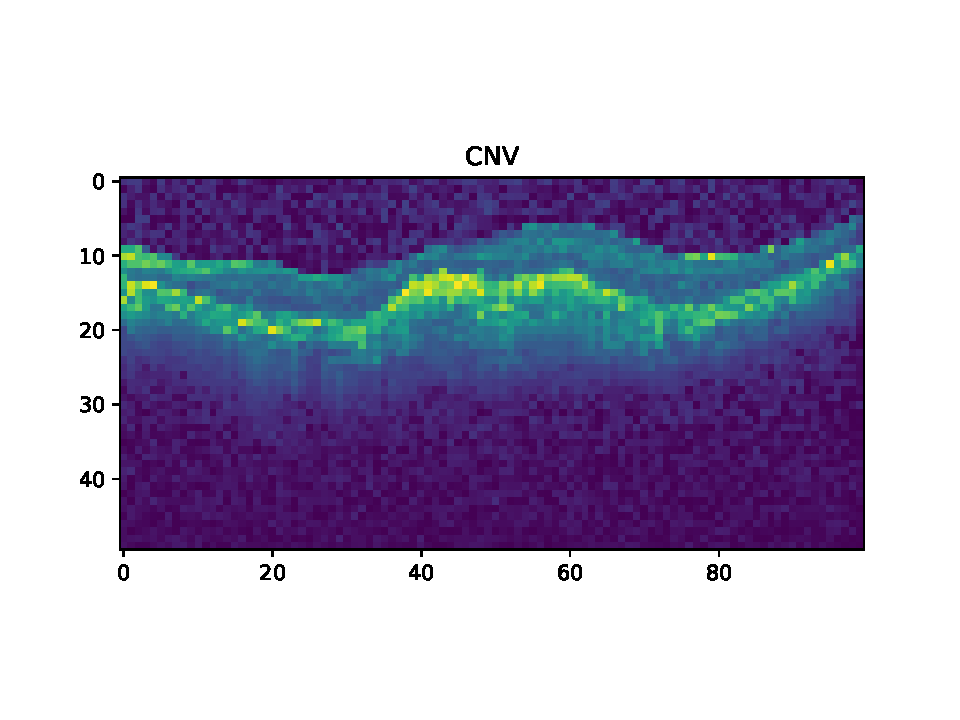
\includegraphics[width=.40\linewidth]{fig/Appendix_DNN/imageCNVscan.pdf}}
\end{subfigure}%
\begin{subfigure}[CNV]{
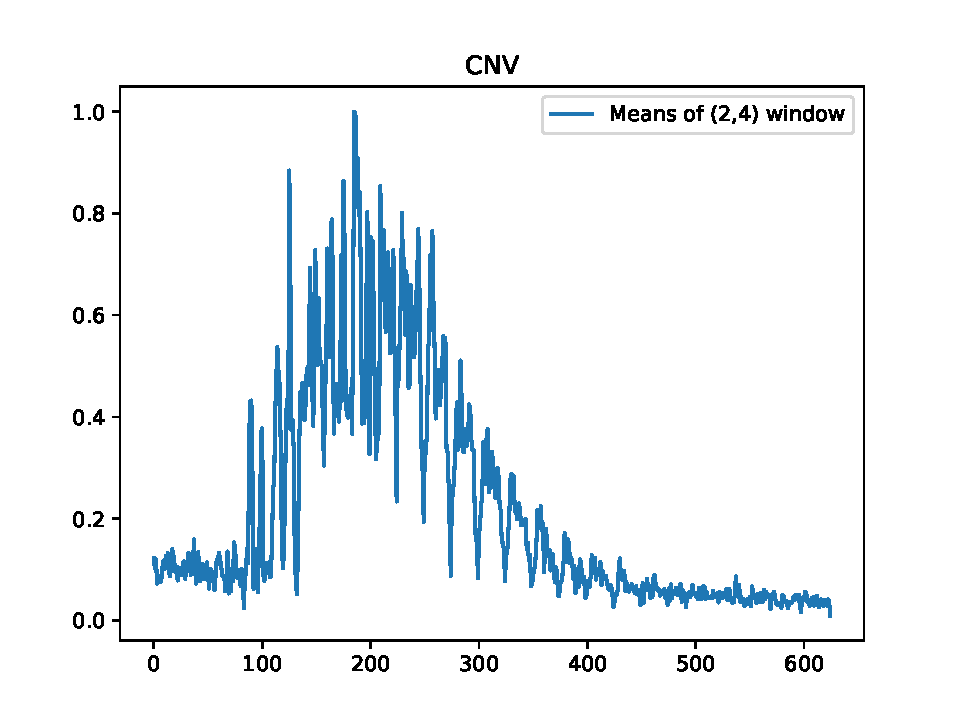
\includegraphics[width=.40\linewidth]{fig/Appendix_DNN/imageCNVmeans.pdf}}
\end{subfigure}\\
\begin{subfigure}[DME]{
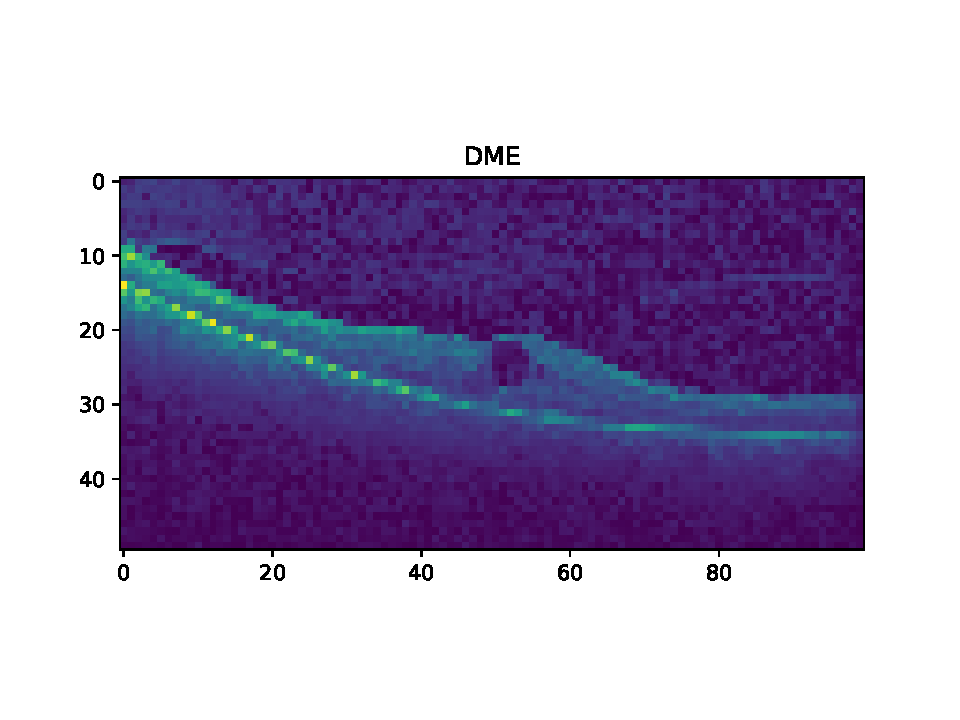
\includegraphics[width=.40\linewidth]{fig/Appendix_DNN/imageDMEscan.pdf}}
\end{subfigure}%
\begin{subfigure}[DME]{
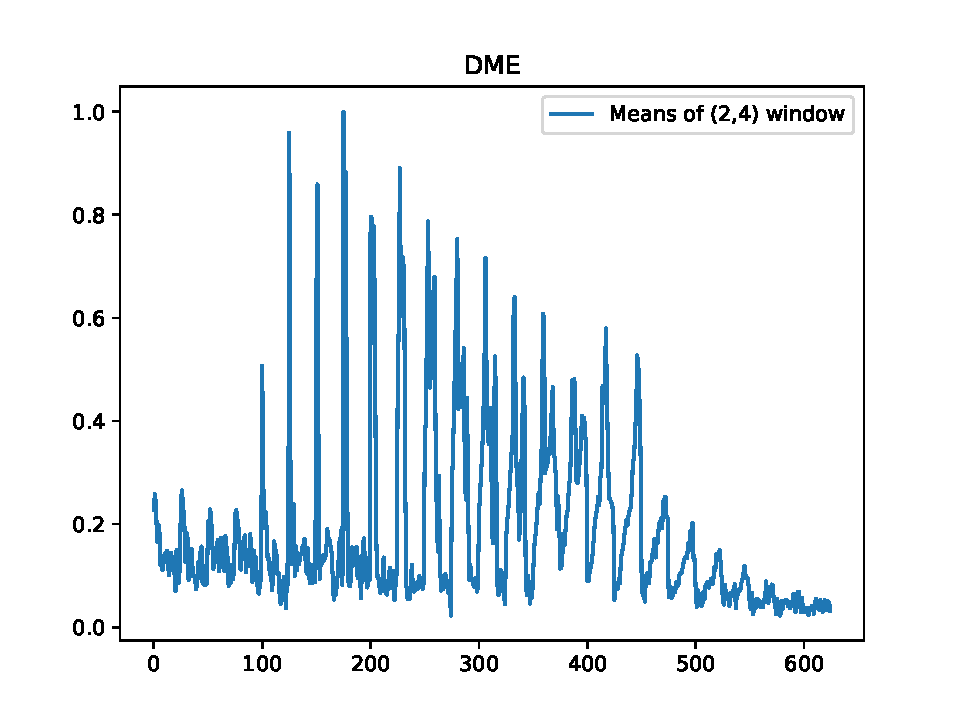
\includegraphics[width=.40\linewidth]{fig/Appendix_DNN/imageDMEmeans.pdf}}
\end{subfigure}\\
\begin{subfigure}[DRUSEN]{
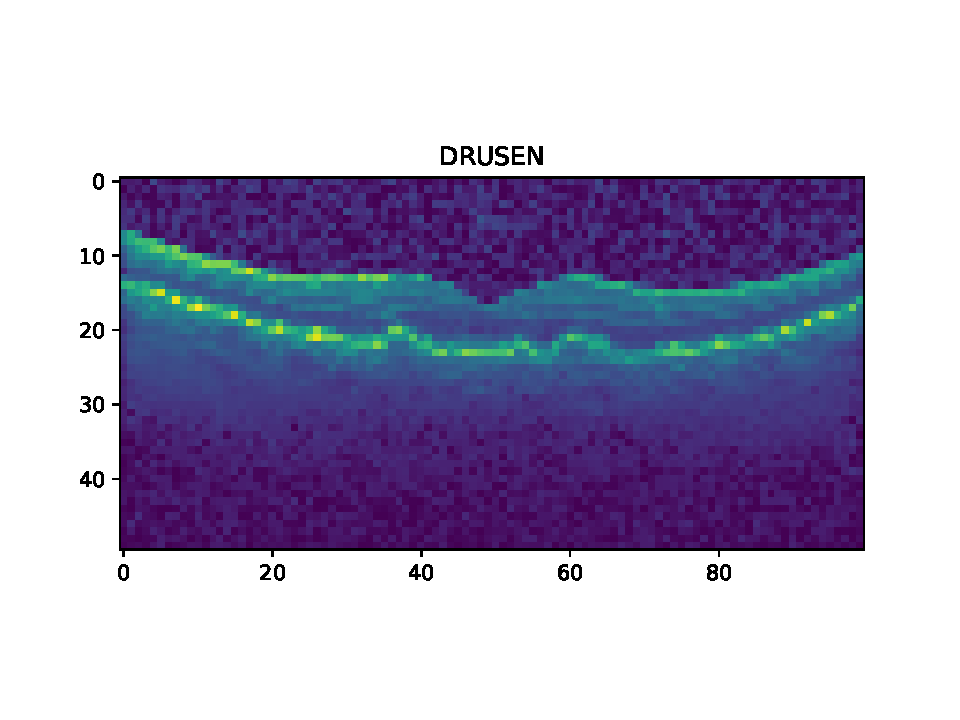
\includegraphics[width=.40\linewidth]{fig/Appendix_DNN/imageDRUSENscan.pdf}}
\end{subfigure}%
\begin{subfigure}[DRUSEN]{
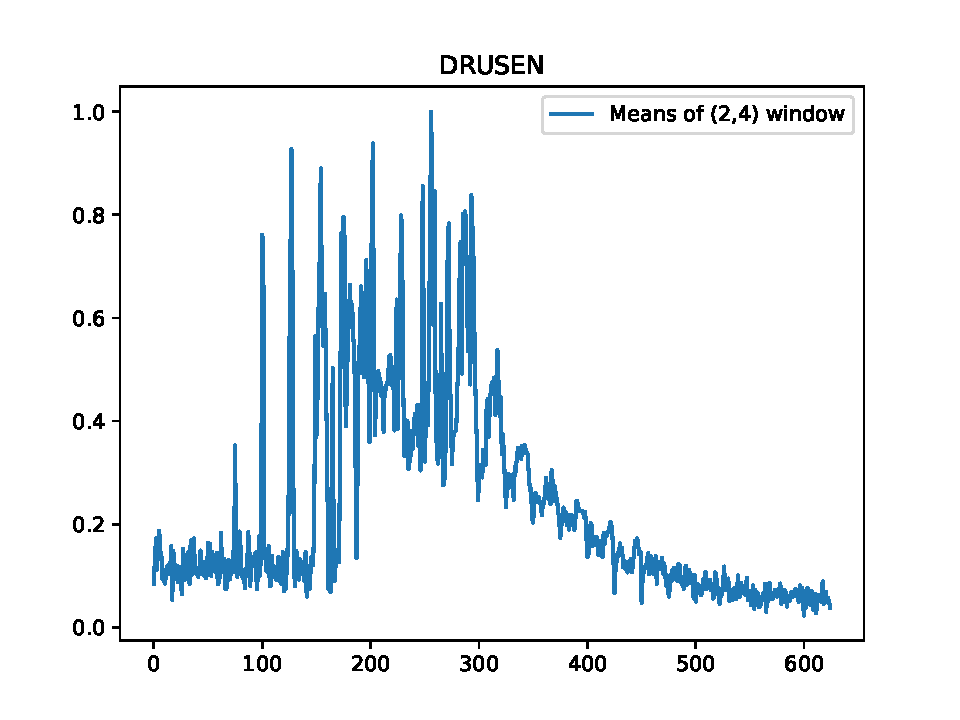
\includegraphics[width=.40\linewidth]{fig/Appendix_DNN/imageDRUSENmeans.pdf}}
\end{subfigure}\\
\caption{Beispielbilder für jede der Klassen im $(50,\,100)$ Format (links) sowie die aus der Abrasterung durch $(2,\,4)$ Fenster erhaltene Verteilung der Mittelwerte (rechts).}
\label{fig:input}
\end{figure}%

\setcounter{subfigure}{0}




\begin{figure}[!t]
 \centering
\begin{subfigure}[Modell 0]{
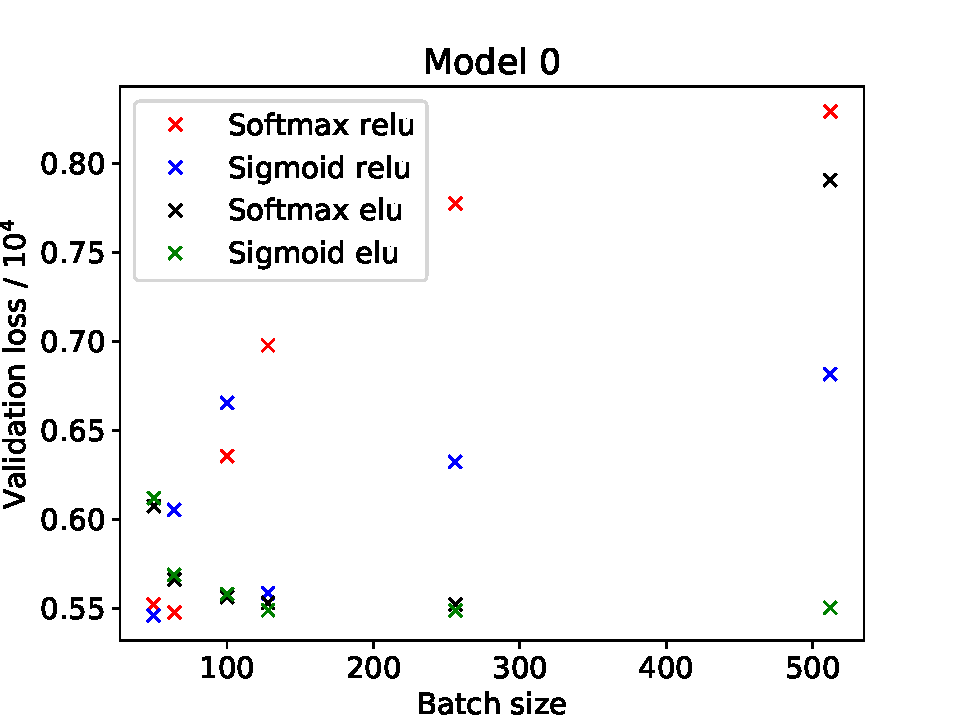
\includegraphics[width=.30\linewidth]{fig/Appendix_DNN/Modelvalloss0.pdf}}
\end{subfigure}%
\begin{subfigure}[Modell 1]{
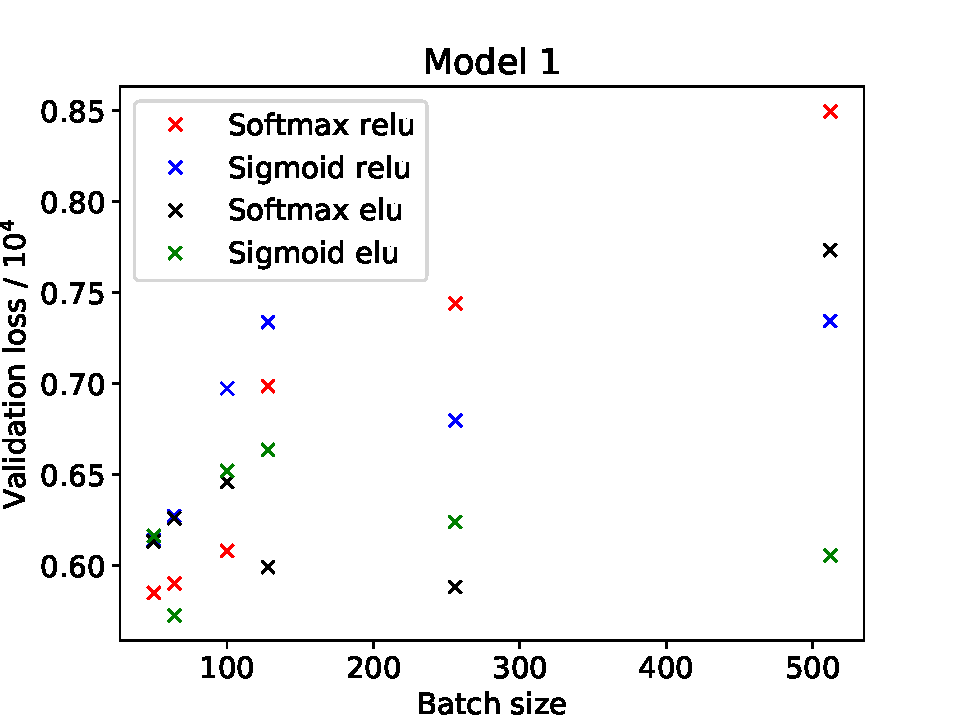
\includegraphics[width=.30\linewidth]{fig/Appendix_DNN/Modelvalloss1.pdf}}
\end{subfigure}
\begin{subfigure}[Modell 2]{
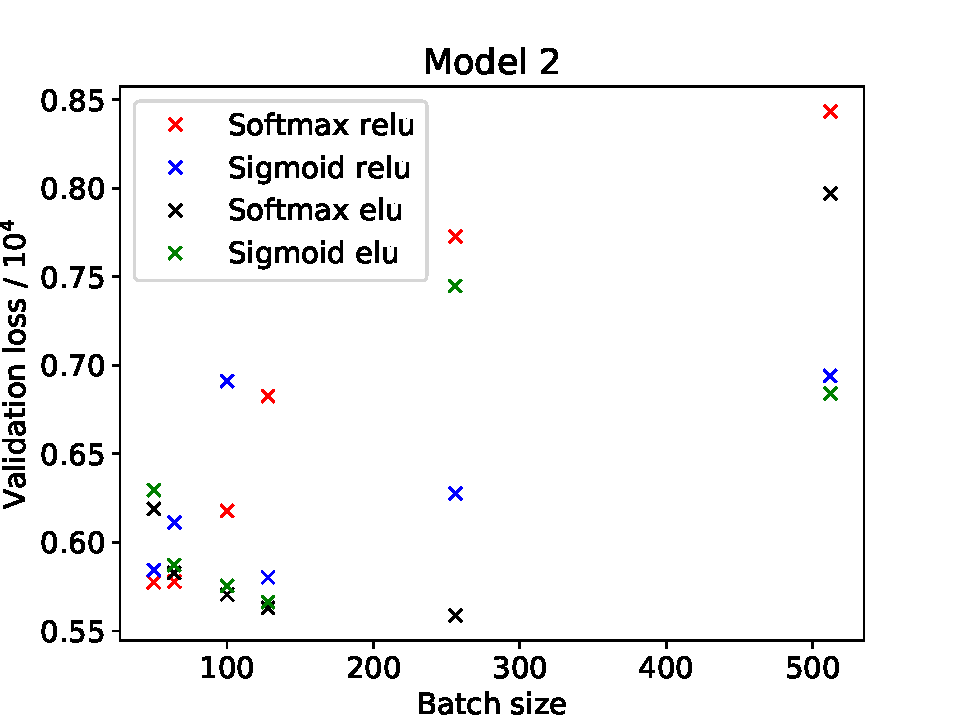
\includegraphics[width=.30\linewidth]{fig/Appendix_DNN/Modelvalloss2.pdf}}
\end{subfigure}\\
\begin{subfigure}[Modell 3]{
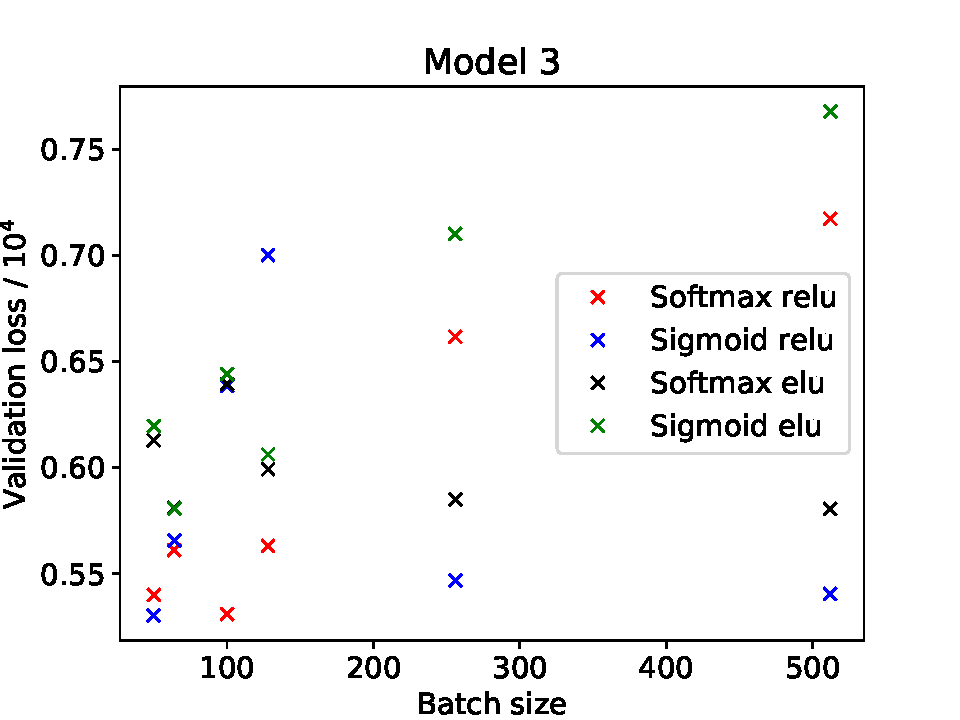
\includegraphics[width=.30\linewidth]{fig/Appendix_DNN/Modelvalloss3.pdf}}
\end{subfigure}
\begin{subfigure}[Modell 4]{
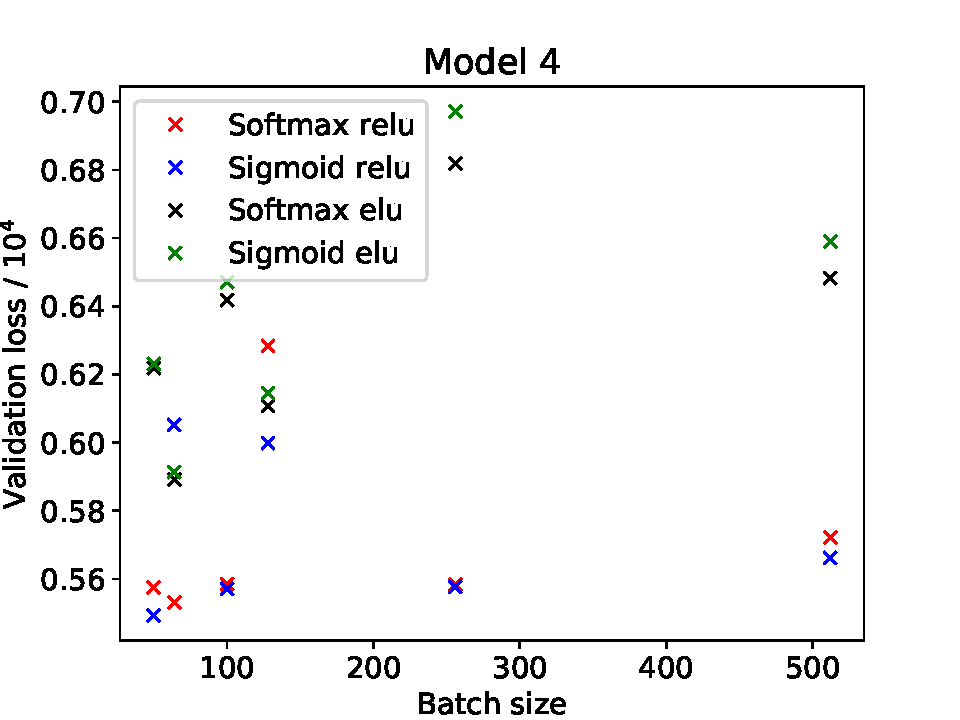
\includegraphics[width=.30\linewidth]{fig/Appendix_DNN/Modelvalloss4.pdf}}
\end{subfigure}
\caption{Erhaltene Werte der Verlustfunktion des DNN für die verschiedenen Konfigurationen der einzelnen Modelle als Funktion der Batch Grö{\ss}e.}
\label{fig:lossgrid}
\end{figure}
\setcounter{subfigure}{0}


\begin{figure}
\centering
 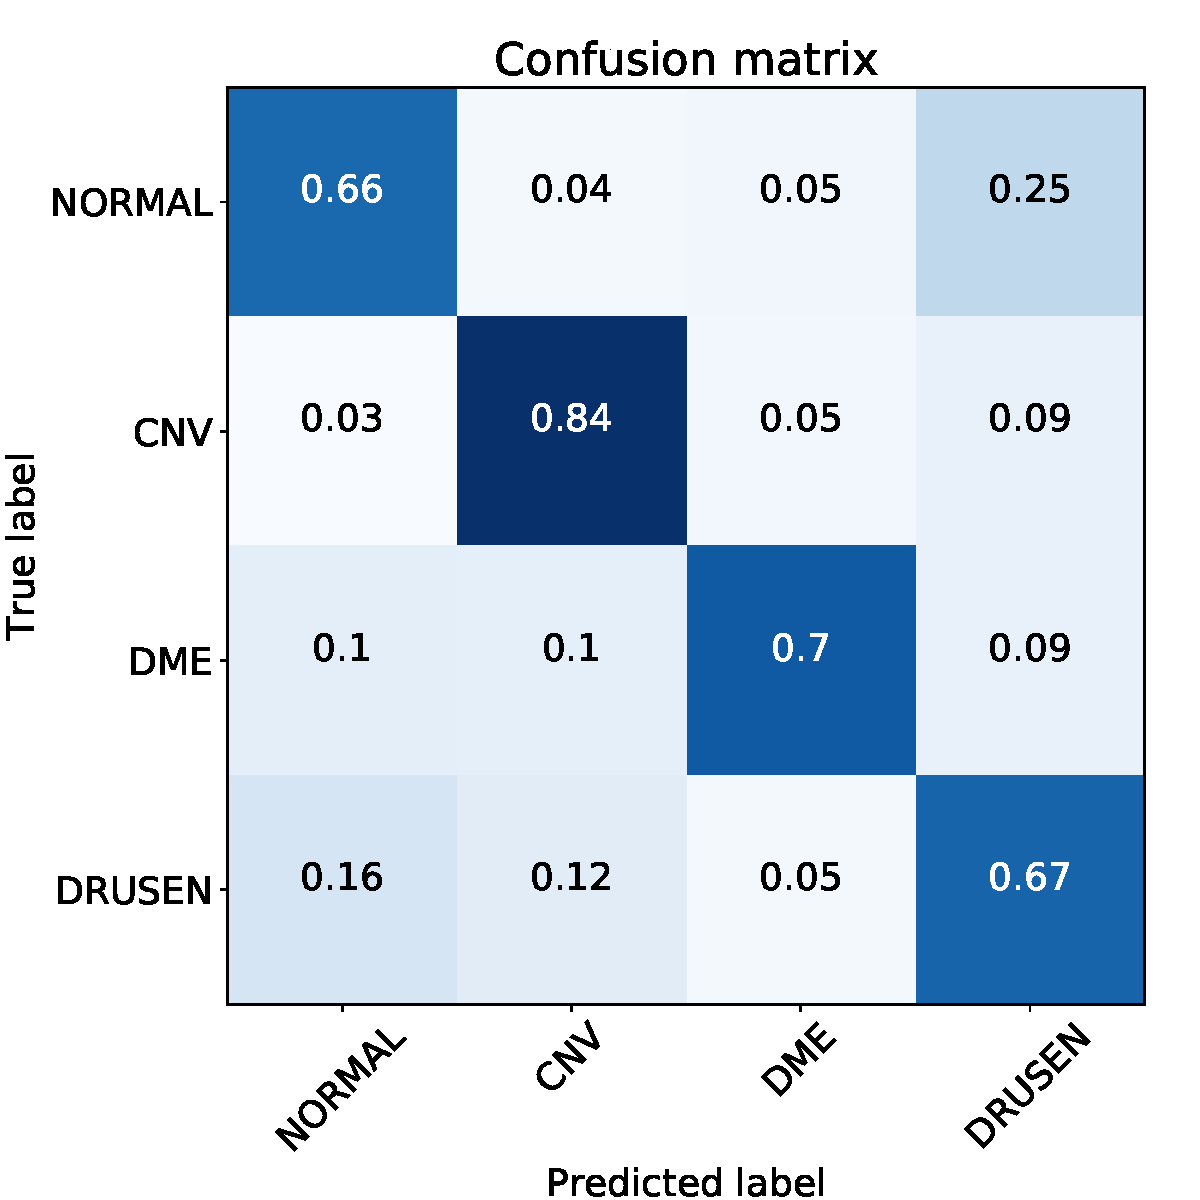
\includegraphics[width=.40\linewidth]{fig/Appendix_DNN/confusionmatrix6.pdf}
 \caption{Verwirrungsmatrix bei Propagation des Valdierungsdatensatzes für die gewählte DNN Struktur.}
\end{figure}
